
\section{PREPARACIÓN DEL ENTORNO DE GENERACIÓN Y CONSTRUCCIÓN}

\subsection{Herramientas y programas usados para el desarrollo}
Para el desarrollo de la aplicación se han utilizado diversas herramientas y programas que han facilitado la creación del sistema.  

\subsubsection{Lenguaje de programación}
El sistema ha sido desarrollado en su totalidad en TypeScript, tanto el \textit{frontend} como el \textit{backend}. 

TypeScript es un superconjunto de JavaScript que añade tipado estático al lenguaje.
Esto permite detectar errores en tiempo de compilación y facilita el mantenimiento del código ya que es mucho más descriptivo.

\begin{figure}[H]
    \centering
    
\includegraphics[width=0.2\textwidth]{figures/7-Construccion/Typescript.png}
    \caption{Logo de TypeScript}
\end{figure}

\subsubsection{Entorno de ejecución}
Se ha utilizado Node.js como entorno de ejecución para JavaScript.
Node.js permite ejecutar código JavaScript en el servidor y es muy popular en el desarrollo de aplicaciones web.
A través de npm, el gestor de paquetes de Node.js, se han instalado las dependencias necesarias para el desarrollo de la aplicación.
Este gestor de paquetes permite instalar y gestionar las dependencias de un proyecto de forma sencilla y cuenta con un amplio repositorio de paquetes.

\begin{figure}[H]
    \centering
    
\includegraphics[width=0.2\textwidth]{figures/7-Construccion/Nodejs.jpeg}
    \caption{Logo de Node.js}
\end{figure}


\subsubsection{Base de datos}
La base de datos utilizada en el sistema es MongoDB, una base de datos NoSQL orientada a documentos.
Se ha utilizado MongoDB Atlas como servicio de base de datos en la nube, lo que ha permitido desplegar la base de datos de forma sencilla y segura.

\begin{figure}[H]
    \centering
    
\includegraphics[width=0.2\textwidth]{figures/7-Construccion/mongodb.png}
    \caption{Logo de MongoDB}
\end{figure}


\subsubsection{Proveedor de servicios en la nube}
Para el despliegue de la aplicación se ha utilizado Azure, la plataforma en la nube de Microsoft.
Azure ofrece una amplia gama de servicios en la nube, como servidores virtuales, bases de datos, almacenamiento y servicios de inteligencia artificial.

\begin{figure}[H]
    \centering
    
\includegraphics[width=0.2\textwidth]{figures/7-Construccion/MicrosoftAzure.png}
    \caption{Logo de Microsoft Azure}
\end{figure}


\subsubsection{Librerías y frameworks}
Se han utilizado diversas librerías y frameworks para el desarrollo de la aplicación, tanto en el \textit{frontend} como en el \textit{backend}.
Este tipo de herramientas permiten acelerar el desarrollo y facilitan la creación de interfaces de usuario y la gestión de la lógica de negocio.
\subsubsection{Frontend}
El \textit{frontend} de la aplicación ha sido desarrollado en React, una librería de JavaScript para la creación de interfaces de usuario,
en combinación con Material-UI, una librería de componentes de React, se ha creado una interfaz de usuario moderna y atractiva.

\begin{figure}[H]
    \centering
    \begin{minipage}{0.3\textwidth}
        \centering
        
\includegraphics[width=\textwidth]{figures/7-Construccion/React.png}
        \caption{Logo de React}
    \end{minipage}
    \hspace{0.05\textwidth}
    \begin{minipage}{0.3\textwidth}
        \centering
        
\includegraphics[width=\textwidth]{figures/7-Construccion/MaterialUI.png}
        \caption{Logo de Material-UI}
    \end{minipage}
\end{figure}


El resto de dependencias que cabe destacar utilizadas en el \textit{frontend} son:
\begin{itemize}
        \item \texttt{redux}: Biblioteca para el manejo del estado de la aplicación.
        \item \texttt{framer-motion}: Librería para animaciones en React.
        \item \texttt{socket.io-client}: Cliente para la comunicación en tiempo real con WebSockets.
        \item \texttt{styled-components}: Librería para escribir CSS en JavaScript.
        \item \texttt{yup}: Librería para la validación de esquemas de datos.
        \item \texttt{sweetalert2}: Librería para mostrar alertas personalizadas.
        \item \texttt{react-router-dom}: Librería para la navegación en React.
        \item \texttt{react-hook-form}: Librería para la gestión de formularios en React.
        \item \texttt{react-paypal-js}: Librería para la integración de pagos con PayPal.
        \item \texttt{react-slick}: Librería para la creación de carruseles en React.
        \item \texttt{Jest}: Framework de pruebas para JavaScript.
        \item \texttt{Puppeteer}: Librería para realizar pruebas de extremo a extremo.
        \item \texttt{Cucumber}: Herramienta para pruebas.
\end{itemize}



\subsubsection{Backend}
El \textit{backend} de la aplicación ha sido desarrollado con Express, un framework de Node.js para la creación de aplicaciones web y APIs.
Express es muy popular en el desarrollo de aplicaciones web y permite crear servidores de forma sencilla y rápida.

\begin{figure}[H]
    \centering
    
\includegraphics[width=0.2\textwidth]{figures/7-Construccion/express.png}
    \caption{Logo de Express}
\end{figure}

Las dependencias más destacadas utilizadas en el \textit{backend} son:
\begin{itemize}
    \item \texttt{axios}: Cliente HTTP basado en promesas para Node.js y el navegador.
    \item \texttt{bcrypt}: Librería para el hashing de contraseñas.
    \item \texttt{body-parser}: Middleware para analizar cuerpos de solicitudes HTTP en Node.js.
    \item \texttt{cors}: Middleware para habilitar CORS (Cross-Origin Resource Sharing).
    \item \texttt{jsonwebtoken}: Implementación de JSON Web Tokens.
    \item \texttt{mongoose}: Librería de modelado de datos de MongoDB para Node.js.
    \item \texttt{socket.io}: Biblioteca para aplicaciones web en tiempo real.
    \item \texttt{yup}: Librería para la validación de esquemas de datos.
    \item \texttt{csv-parser}: Librería para analizar archivos CSV.
    \item \texttt{csv-writer}: Librería para escribir archivos CSV.
    \item \texttt{paypal-rest-sdk}: SDK para la integración con PayPal.
    \item \texttt{Jest}: Framework de pruebas para JavaScript.
    \item \texttt{supertest}: Biblioteca para pruebas HTTP.
\end{itemize}



\subsubsection{Entorno de desarrollo}
\subsubsubsection{Gestión de versiones}
Para la gestión de versiones se ha utilizado Git, un sistema de control de versiones distribuido que permite llevar un control de los cambios en el código fuente.
Como plataforma de alojamiento de repositorios se ha utilizado GitHub, que permite alojar proyectos de software y facilita la colaboración entre desarrolladores.
Además, se ha utilizado GitHub Actions para la integración continua y GitKraken como cliente de escritorio para la gestión de ramas y \textit{pull requests}.


\begin{figure}[H]
    \centering
    \begin{minipage}{0.2\textwidth}
        \centering
        
\includegraphics[width=\textwidth]{figures/7-Construccion/Git.png}
        \caption{Logo de Git}
    \end{minipage}
    \hfill
    \begin{minipage}{0.2\textwidth}
        \centering
        
\includegraphics[width=\textwidth]{figures/7-Construccion/Github.png}
        \caption{Logo de GitHub}
    \end{minipage}
    \hfill
    \begin{minipage}{0.3\textwidth}
        \centering
        
\includegraphics[width=\textwidth]{figures/7-Construccion/GitKraken.jpeg}
        \caption{Logo de GitKraken}
    \end{minipage}
\end{figure}

\subsubsubsection{Editor de código}
Para el desarrollo del código fuente se ha utilizado Visual Studio Code, 
un editor de código fuente desarrollado por Microsoft que incluye soporte para depuración, control de versiones y resaltado de sintaxis.
Admite extensiones que permiten ampliar sus funcionalidades y es muy popular entre los desarrolladores.

\begin{figure}[H]
    \centering
    \includegraphics[width=0.2\textwidth]{figures/7-Construccion/VSCode.png}
    \caption{Logo de Visual Studio Code}
\end{figure}

Además, se ha utilizado Notepad++ como editor de texto para la edición de archivos de configuración y otros archivos de texto
necesarios para desplegar la aplicación en un servidor.

\begin{figure}[H]
    \centering
    
\includegraphics[width=0.2\textwidth]{figures/7-Construccion/Notepad.png}
    \caption{Logo de Notepad++}
\end{figure}


\subsubsection{Cliente SSH}
Para la conexión remota con el servidor se ha utilizado MobaXterm, un cliente SSH que permite conectarse a servidores remotos de forma segura.
Tiene una interfaz gráfica intuitiva y permite la transferencia de archivos a través de SCP y SFTP.
Se ha utilizado principalmente para la conexión con el servidor de producción y para la transferencia de archivos.

\begin{figure}[H]
    \centering
    \includegraphics[width=0.2\textwidth]{figures/7-Construccion/MobaXterm.png}
    \caption{Logo de MobaXterm}
\end{figure}

\subsubsection{Postman}
Para probar las rutas de la API se ha utilizado Postman, una herramienta que permite realizar peticiones HTTP a servidores y analizar las respuestas.
De esta manera se ha comprobado el funcionamiento de la API sin necesidad de utilizar el \textit{frontend}, lo que ha facilitado el desarrollo y la depuración de la aplicación.

\begin{figure}[H]
    \centering
    \includegraphics[width=0.2\textwidth]{figures/7-Construccion/Postman.png}
    \caption{Logo de Postman}
\end{figure}


\subsubsection{Documentación}

\subsubsubsection{Memoria del proyecto}
La documentación del proyecto se ha realizado con LaTeX, un sistema de composición de textos que permite crear documentos de alta calidad tipográfica.
Se ha utilizado la herramienta Overleaf para la visualización y edición de los documentos, ya que permite la colaboración en tiempo real y la exportación a PDF.


\begin{figure}[H]
    \centering
    \begin{minipage}{0.2\textwidth}
        \centering
        
\includegraphics[width=\textwidth]{figures/7-Construccion/LaTeX.png}
        \caption{Logo de LaTeX}
    \end{minipage}
    \hspace{0.05\textwidth}
    \begin{minipage}{0.2\textwidth}
        \centering
        \includegraphics[width=\textwidth]{figures/7-Construccion/Overleaf.png}
        \caption{Logo de Overleaf}
    \end{minipage}
\end{figure}


\subsubsubsection{Diagramas}
Para la creación de diagramas se han utilizado diversas herramientas, como Lucidchart y Draw.io, que permiten crear diagramas de forma sencilla y exportarlos en varios formatos.
Se ha utilizado PlantUML para la creación de diagramas de forma textual, lo que facilita la creación y modificación de los diagramas. 
Por último, se ha utilizado Excalidraw para la creación de las interfaces de usuario de la aplicación.

\begin{figure}[H]
    \centering
    \begin{minipage}{0.2\textwidth}
        \centering
        
\includegraphics[width=\textwidth]{figures/7-Construccion/Lucidchart.png}
        \caption{Logo de Lucidchart}
    \end{minipage}
    \hspace{0.05\textwidth}
    \begin{minipage}{0.2\textwidth}
        \centering
        \includegraphics[width=\textwidth]{figures/7-Construccion/Drawio.png}
        \caption{Logo de Draw.io}
    \end{minipage}
\end{figure}

\begin{figure}[H]
    \centering
    \begin{minipage}{0.2\textwidth}
        \centering
        \includegraphics[width=\textwidth]{figures/7-Construccion/PlantUML.png}
        \caption{Logo de PlantUML}
    \end{minipage}
    \hspace{0.05\textwidth}
    \begin{minipage}{0.2\textwidth}
        \centering
        
\includegraphics[width=\textwidth]{figures/7-Construccion/Exacalidraw.jpeg}
        \caption{Logo de Excalidraw}
    \end{minipage}
\end{figure}


\subsubsubsection{Hojas de cálculo}
Para la creación de hojas de cálculo se ha utilizado Microsoft Excel, una herramienta de Microsoft Office que permite crear y editar hojas de cálculo.
Se ha utilizado principalemente para la elaboración de presupuestos y cálculos de costes.

\begin{figure}[H]
    \centering
    
\includegraphics[width=0.2\textwidth]{figures/7-Construccion/Excel.png}
    \caption{Logo de Microsoft Excel}
\end{figure}

\subsubsubsection{Planificación}
Para la planificación del proyecto se ha utilizado Microsoft Project, una herramienta de Microsoft Office que permite crear diagramas de Gantt y planificar tareas y recursos.
Se ha utilizado para la planificación del proyecto y el seguimiento de las tareas.

\begin{figure}[H]
    \centering
    
\includegraphics[width=0.2\textwidth]{figures/7-Construccion/Project.png}
    \caption{Logo de Microsoft Project}
\end{figure}



\newpage
\section{ELABORACIÓN DE LOS MANUALES DE USUARIO}

\subsection{Manual de Instalación y Ejecución}
El código fuente de la aplicación se encuentra en el repositorio de GitHub \coloredUnderline{\href{https://github.com/paulasuarezp/BidMonUniverse}{BidMonUniverse}}.
por lo que para instalar la aplicación es necesario clonar el repositorio en un entorno local.

Para instalar la aplicación en un entorno local, se deben seguir los siguientes pasos:
\begin{enumerate}
    \item Clonar el repositorio de GitHub en un entorno local.
    \item Instalar Node.js y npm en el sistema.
    \begin{itemize}
        \item Para instalar Node.js se puede descargar el instalador desde la página oficial de Node.js \coloredUnderline{\href{https://nodejs.org/en/download/prebuilt-installer}{nodejs.org}}.
        \item npm se instala automáticamente con Node.js.
        \item Para comprobar que Node.js y npm se han instalado correctamente, se puede ejecutar el siguiente comando en una terminal:
        \begin{itemize}
            \item \texttt{node -v}
            \item \texttt{npm -v}
        \end{itemize}
    \end{itemize}

    \item Instalar las dependencias de \textit{webapp}. Para ello hay que ejecutar los siguientes comandos:
      \begin{enumerate}
          \item \texttt{cd webapp}
          \item \texttt{npm install}
      \end{enumerate}
    \item Instalar las dependencias de \textit{restapi}. Para ello hay que ejecutar los siguientes comandos:
      \begin{enumerate}
          \item \texttt{cd restapi}
          \item \texttt{npm install}
      \end{enumerate}
    \item Configurar las variables de entorno.
      \begin{enumerate}
          \item Crear un archivo \texttt{.env} en la carpeta \texttt{restapi} con las siguientes variables de entorno:
          \begin{itemize}
              \item \texttt{MONGO\_URI}: URI de la base de datos de MongoDB.
              \item \texttt{TOKEN\_SECRET}: Clave secreta para la generación de tokens JWT.
              \item \texttt{TEST\_MONGO\_URI}: URI de la base de datos de pruebas de MongoDB.
              \item \texttt{PAYPAL\_CLIENT\_ID}: ID de cliente de PayPal.
              \item \texttt{PAYPAL\_CLIENT\_SECRET}: Clave secreta de PayPal.
              \item \texttt{NODE\_ENV=development}: Entorno de desarrollo.
          \end{itemize}

    \item Iniciar la aplicación. Para ello hay que ejecutar los siguientes comandos:
      \begin{enumerate}
          \item \texttt{cd backend}, si no se está en la carpeta del \textit{backend}.
          \item \texttt{npm start}
          \item \texttt{cd frontend}, si no se está en la carpeta del \textit{frontend}.
          \item \texttt{npm start}
      \end{enumerate}
    \item Acceder a la aplicación en un navegador web a través de la dirección \texttt{http://localhost:3000}.
\end{enumerate}


\subsection{Manual de Usuario} 
El manual de usuario describe las funcionalidades de la aplicación y cómo utilizarlas.
Se divide en varias secciones, cada una de las cuales describe una parte de la aplicación y cómo interactuar con ella.

\subsubsection{Inicio de sesión}
Para acceder a la aplicación es necesario iniciar sesión con un usuario y una contraseña.
Si no se dispone de una cuenta, se puede crear una nueva cuenta pulsando en el enlace de registro.
Una vez iniciada la sesión, se accede a la página principal de la aplicación.
El usuario recibe como bienvenida 100 Zens, la moneda virtual de la aplicación, que se pueden utilizar para comprar sobres de cartas
y participar en subastas.

\begin{figure}[H]
    \centering
    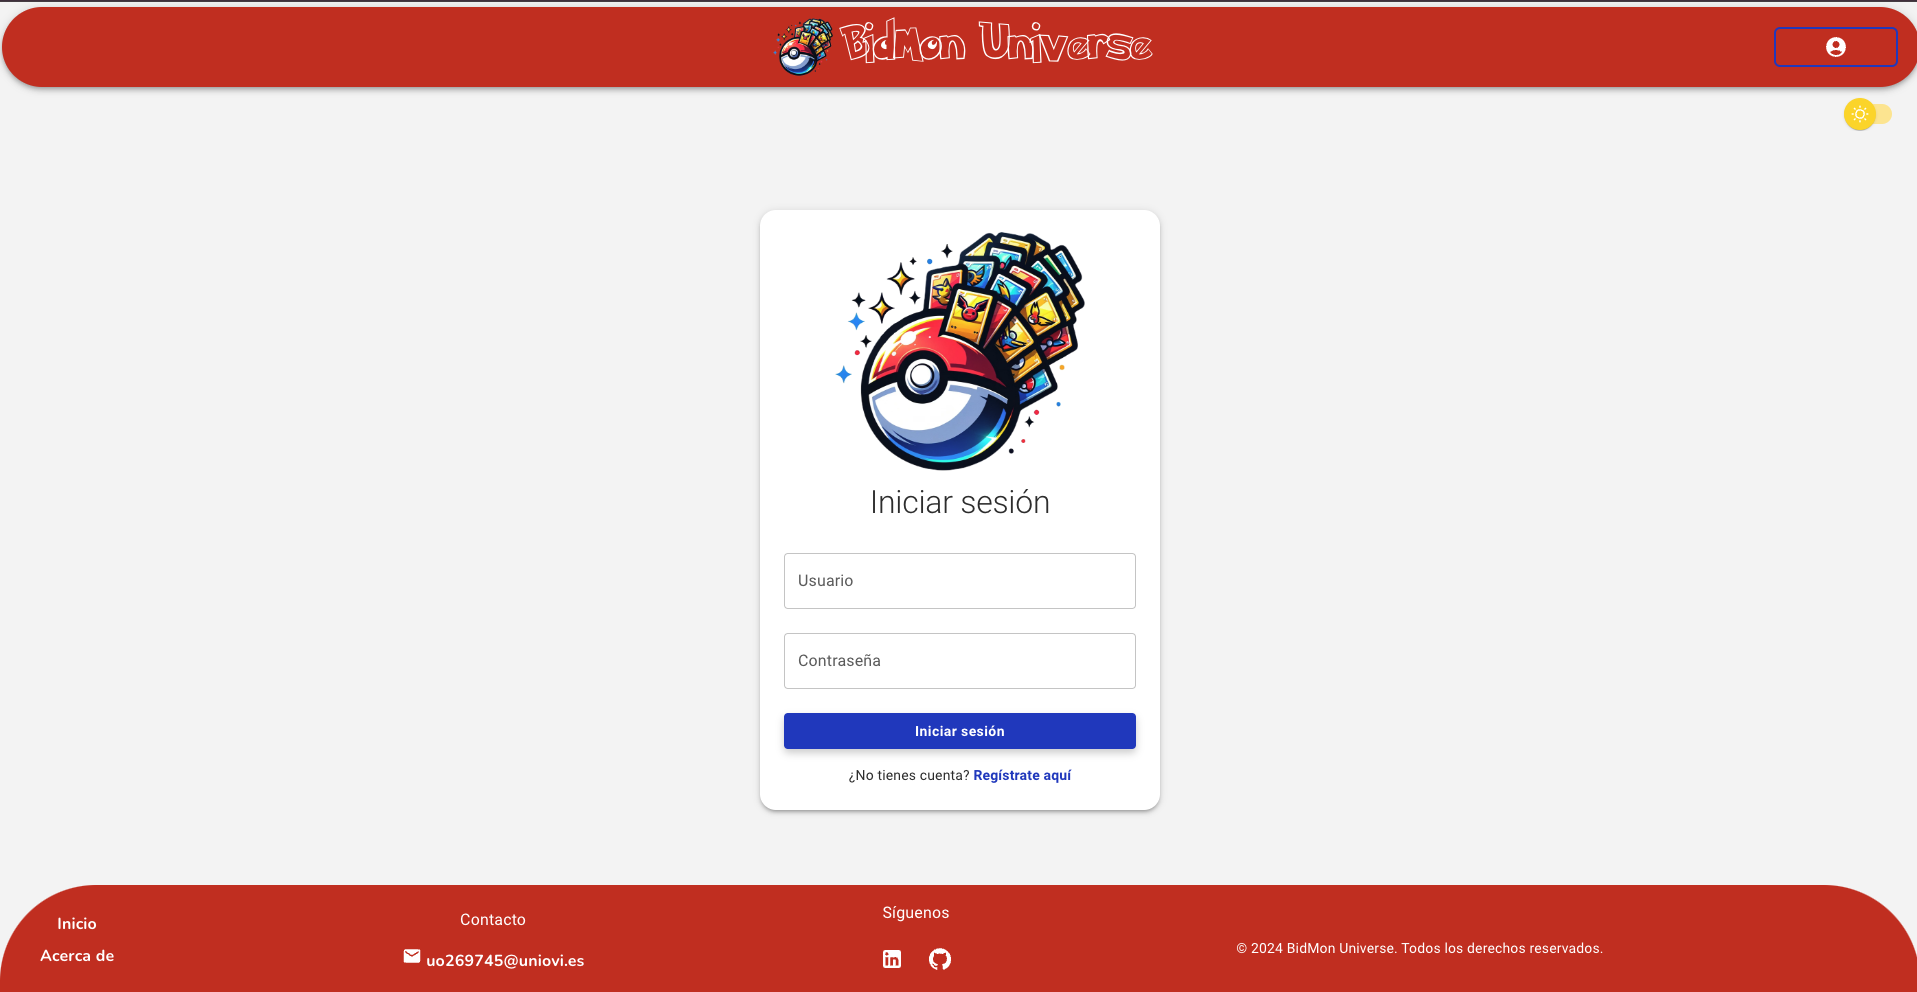
\includegraphics[width=0.8\textwidth]{figures/6-Analisis/6-Interfaz/interfaz/login.png}
    \caption{Página de inicio de sesión.}
    \label{fig:m-interfaz-login}
\end{figure}


\subsubsection{Registro}
Para registrarse en la aplicación es necesario introducir un nombre de usuario, la fecha de nacimiento y una contraseña.
Los usuarios menores de 18 años no pueden registrarse en la aplicación.
Una vez completado el registro, se puede iniciar sesión con el nuevo usuario y acceder a la página principal de la aplicación.

\begin{figure}[H]
    \centering
    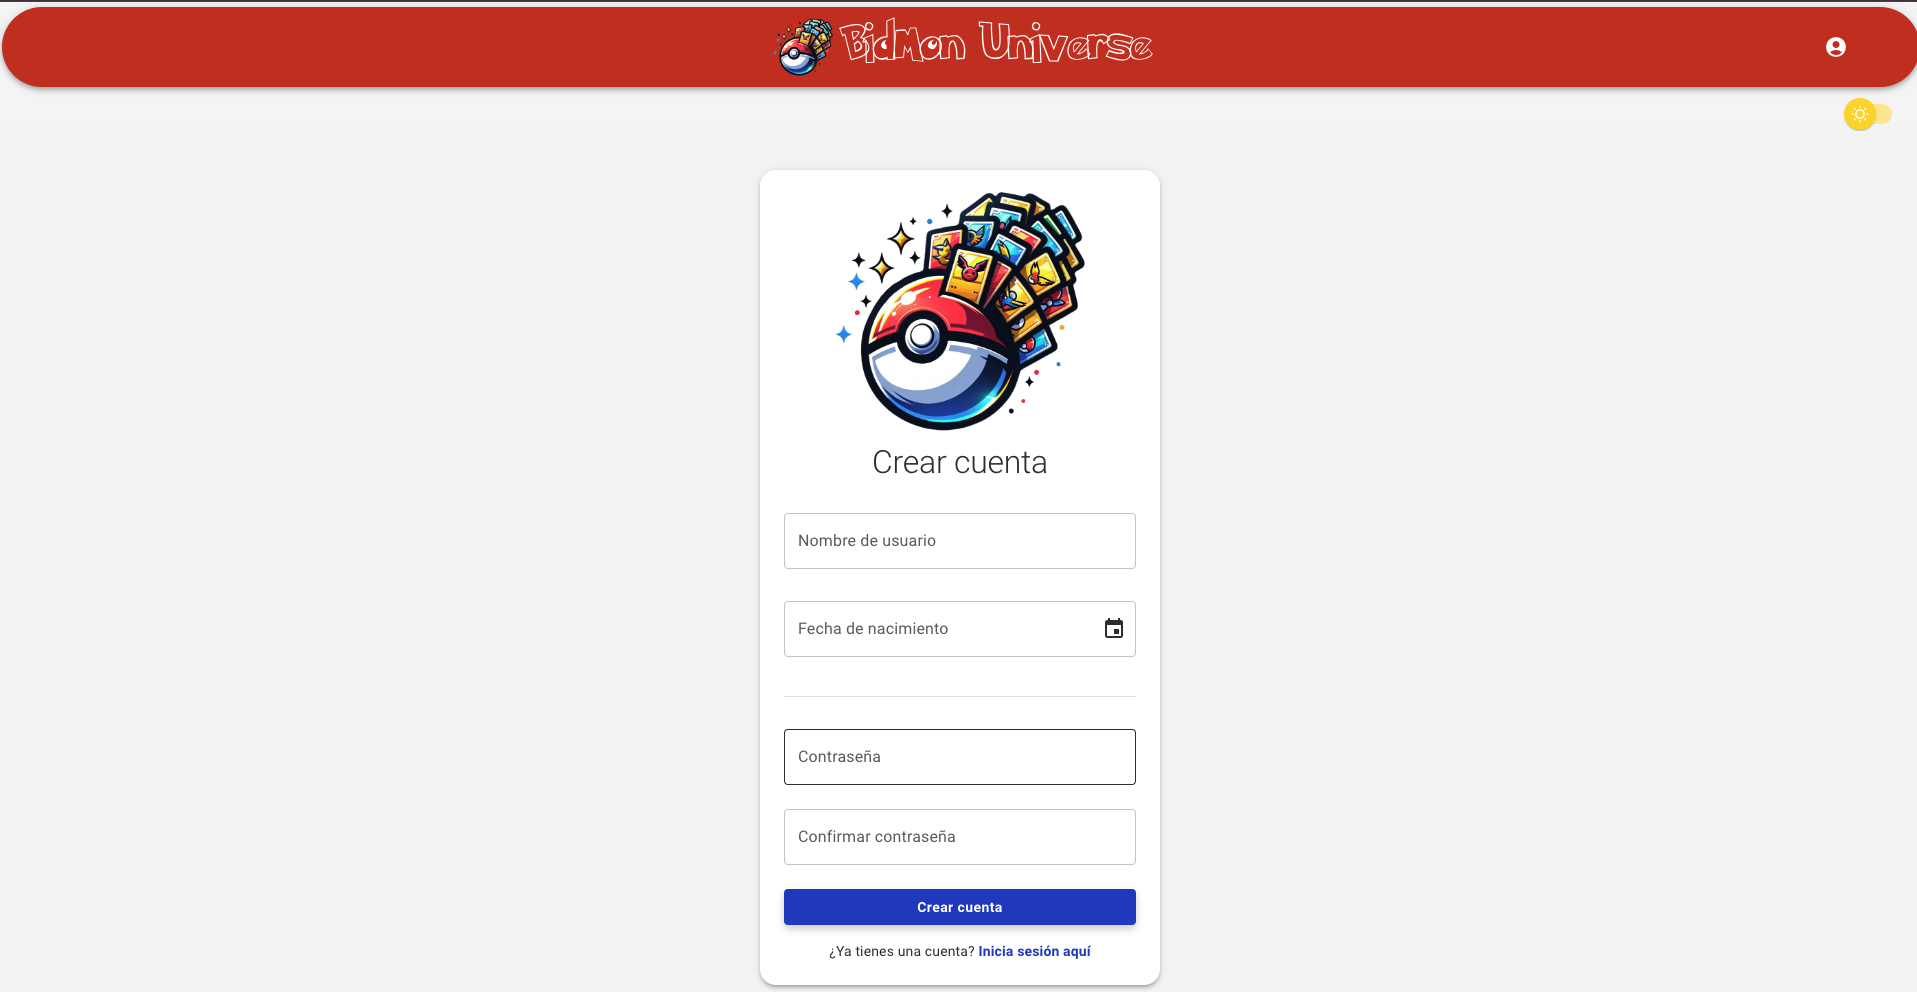
\includegraphics[width=0.8\textwidth]{figures/6-Analisis/6-Interfaz/interfaz/signup.png}
    \caption{Página de registro de usuario.}
    \label{fig:m-interfaz-registro}
\end{figure}


\subsubsection{Página principal}
En la página principal podemos consultar un resumen de la colección de cartas del usuario, el saldo de Zens y un resumen
de las subastas que el usuario ha creado así como un resumen de las pujas activas.
Desde esta página se puede acceder a las diferentes secciones de la aplicación, como la colección de cartas, las subastas, la tienda
y el histórico de transacciones.

\begin{figure}[H]
    \centering
    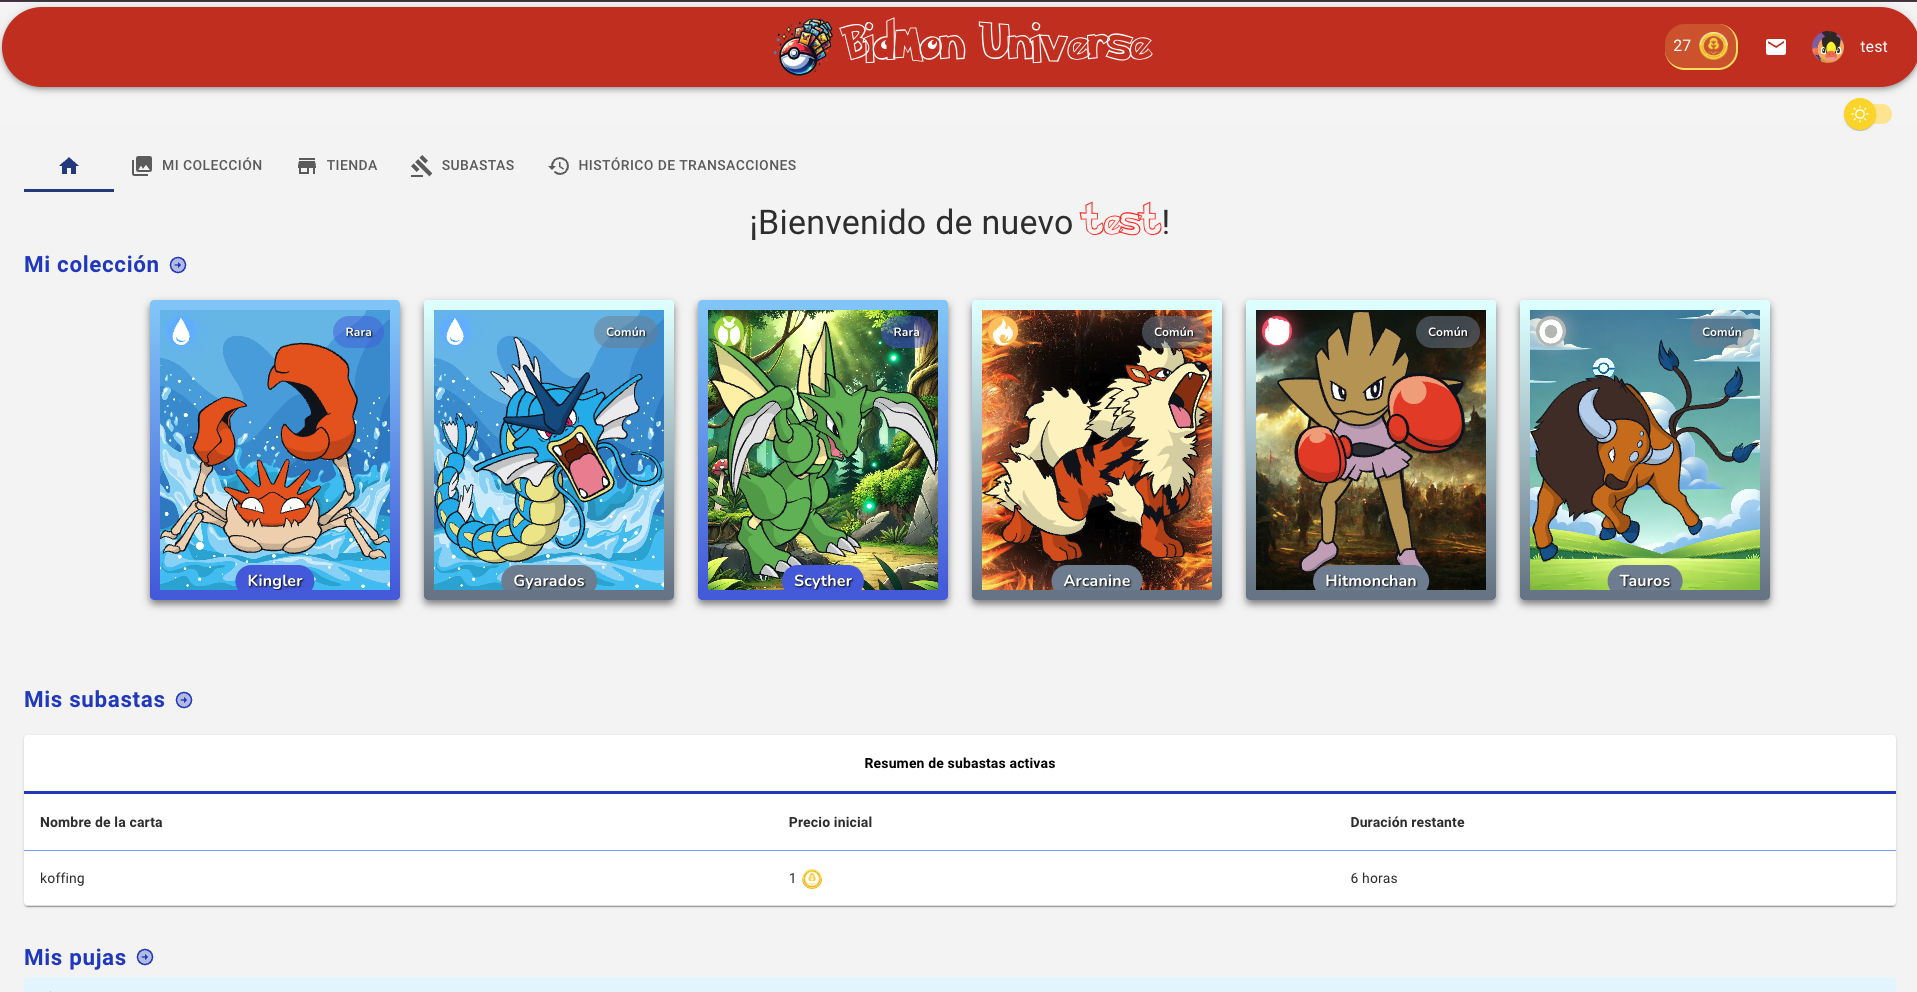
\includegraphics[width=0.8\textwidth]{figures/6-Analisis/6-Interfaz/interfaz/logued.png}
    \caption{Página principal de la aplicación, una vez que el usuario ha iniciado sesión.}
    \label{fig:m-interfaz-logued}
\end{figure}

\subsubsection{Compra de cartas}
En la tienda se pueden comprar sobres de cartas con Zens.
Cada sobre contiene un número determinado de cartas, que se añaden a la colección del usuario.
Estas cartas se pueden vender en subastas.

\begin{figure}[H]
    \centering
    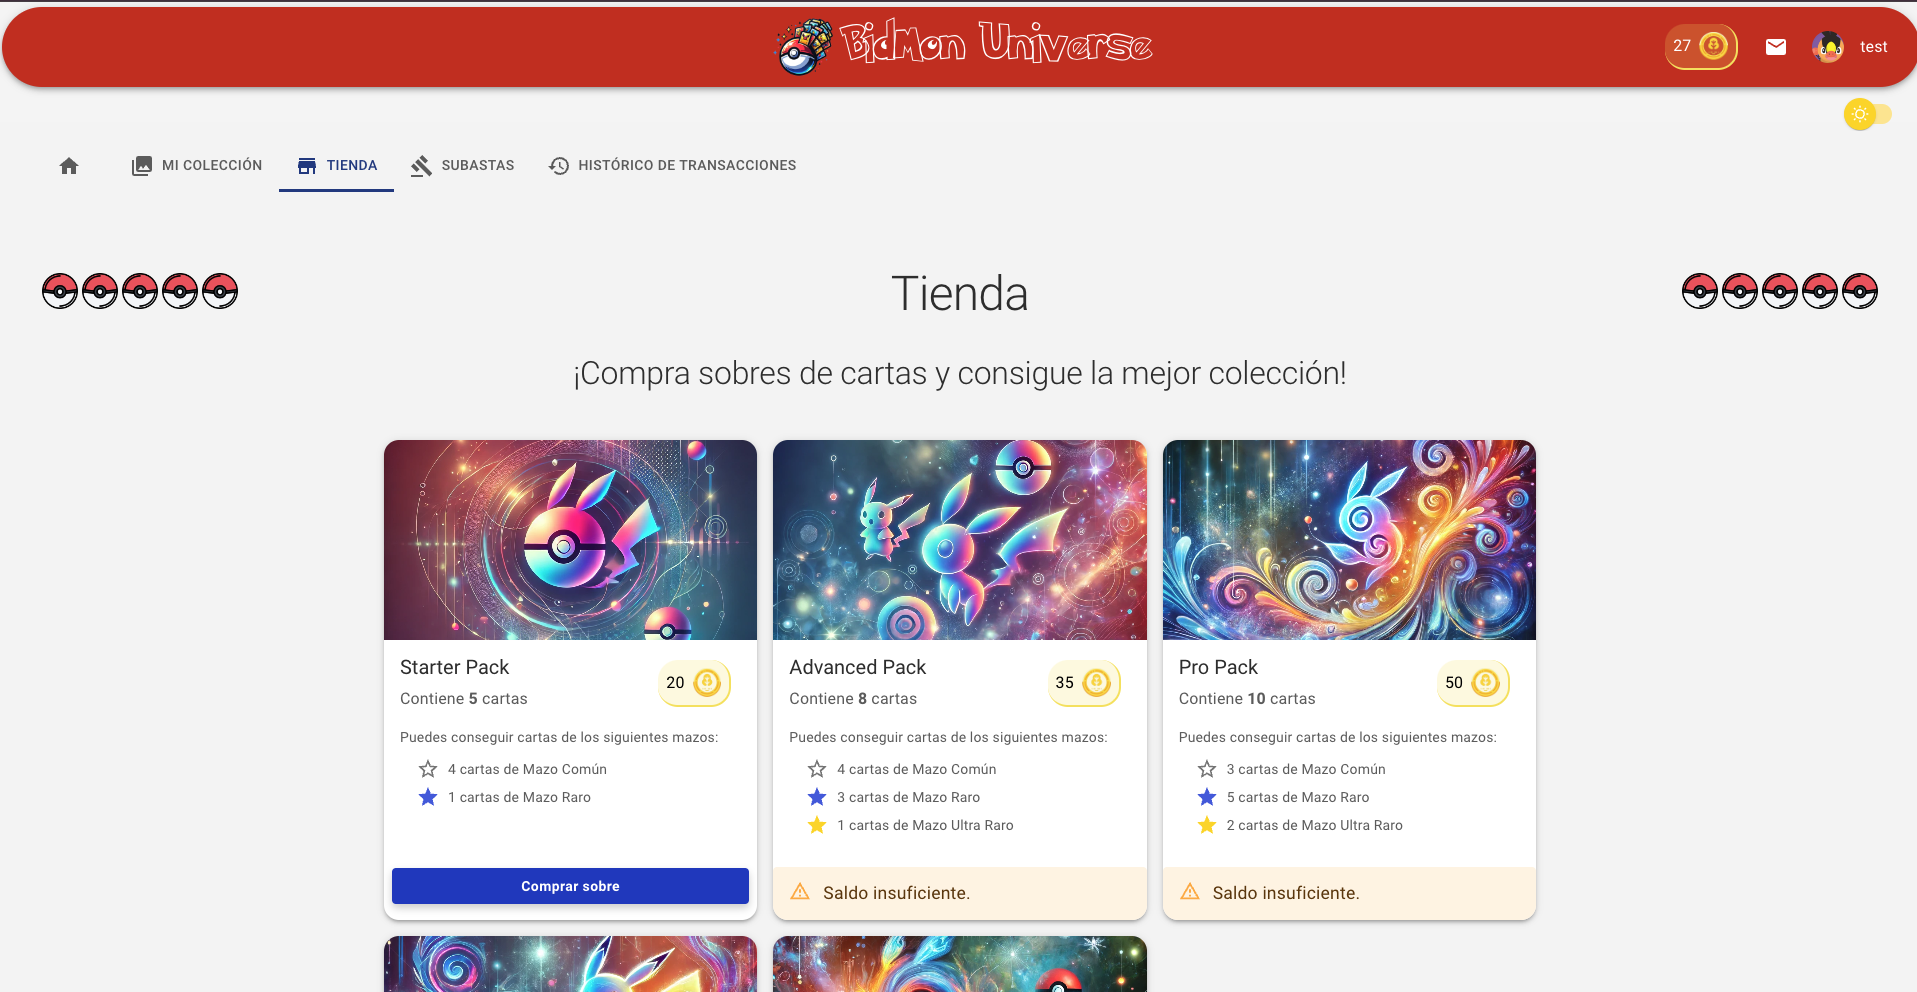
\includegraphics[width=0.8\textwidth]{figures/6-Analisis/6-Interfaz/interfaz/tienda.png}
    \caption{Página de la tienda de sobres de cartas.}
    \label{fig:m-interfaz-tienda}
\end{figure}

Cuando el usuario compra un sobre, se le muestran las cartas que ha adquirido.
Para simular la compra de un sobre real, las cartas aparecen inicialmente boca abajo y es el usuario quien
tiene que hacer clic en cada carta para que esta se dé la vuelta y se muestre.

\begin{figure}[H]
    \centering
    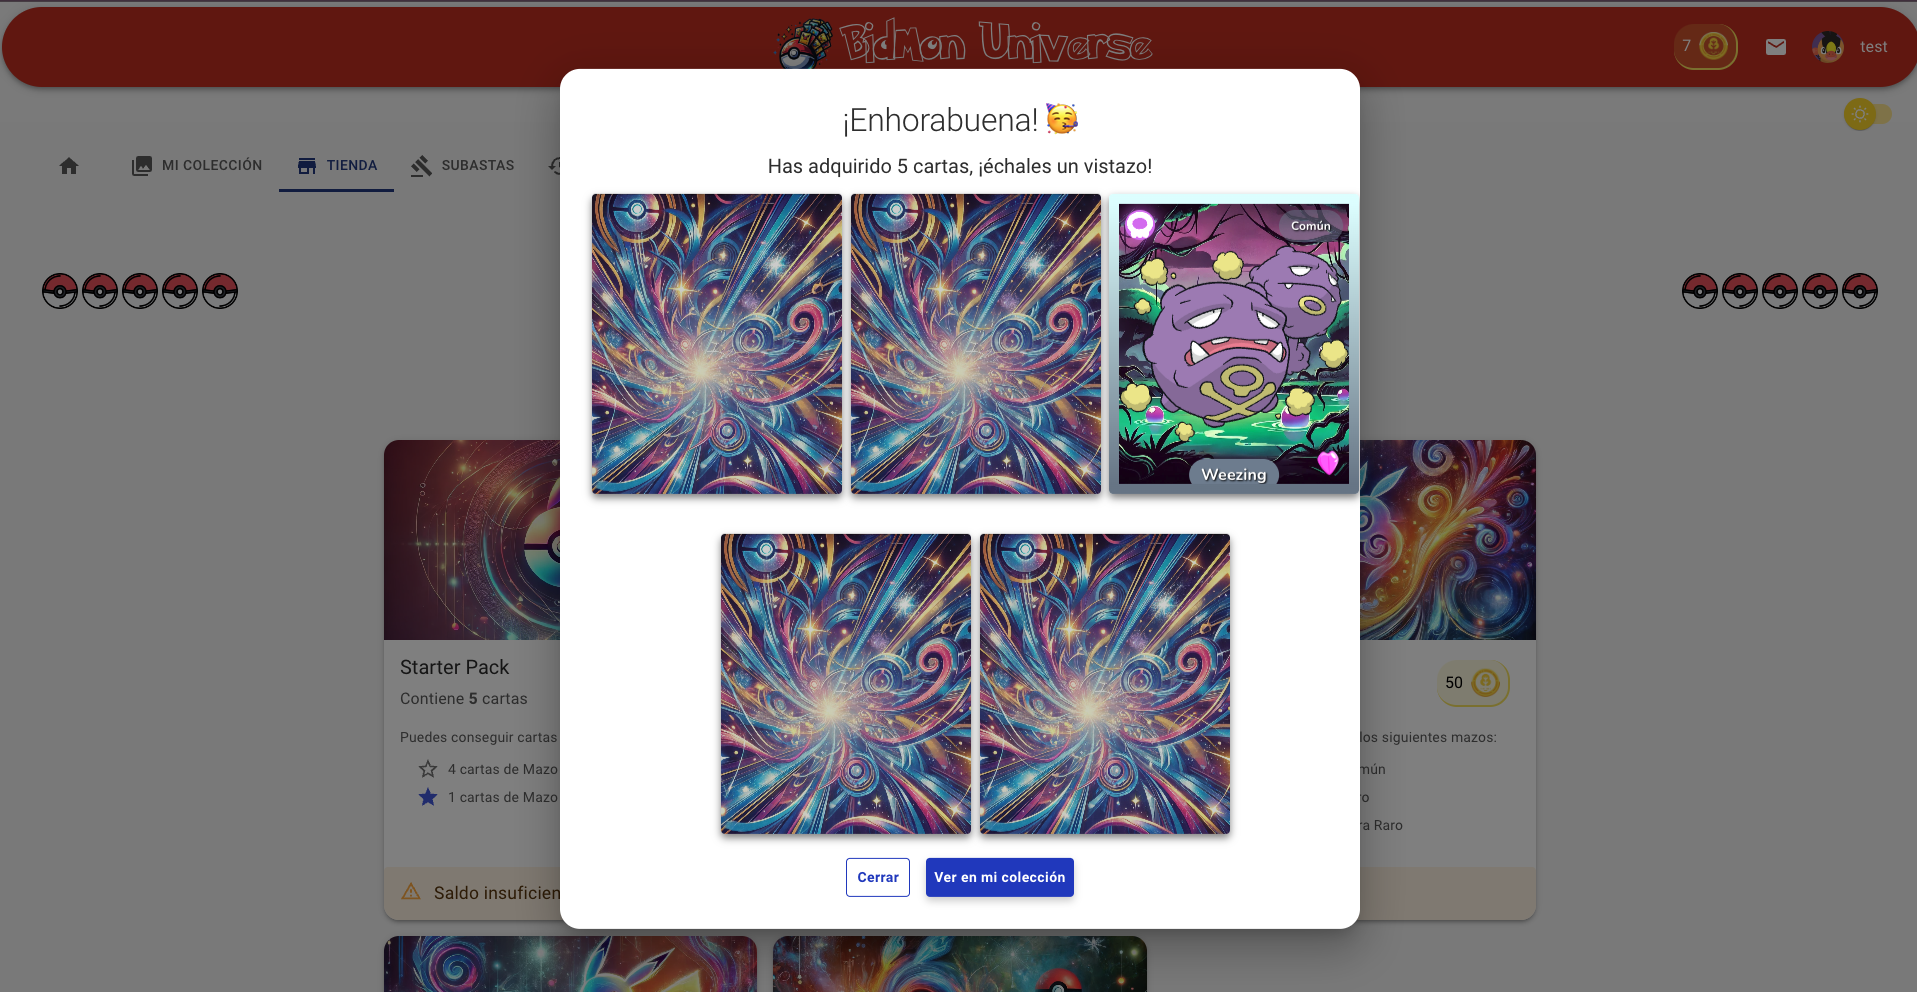
\includegraphics[width=0.8\textwidth]{figures/6-Analisis/6-Interfaz/interfaz/compra_sobre.png}
    \caption{Modal de cartas obtenidas en el sobre.}
    \label{fig:m-interfaz-sobre-comprado}
\end{figure}

Una vez que el usuario ha adquirido las cartas, puede verlas en la colección de cartas.


\subsubsection{Colección de cartas}
En la colección de cartas se pueden ver todas las cartas que el usuario ha adquirido.
Si se hace clic en una carta, se muestra un detalle de la carta con información adicional, como el nombre, el tipo, la rareza y
el historial de transacciones de la carta.

\begin{figure}[H]
    \centering
    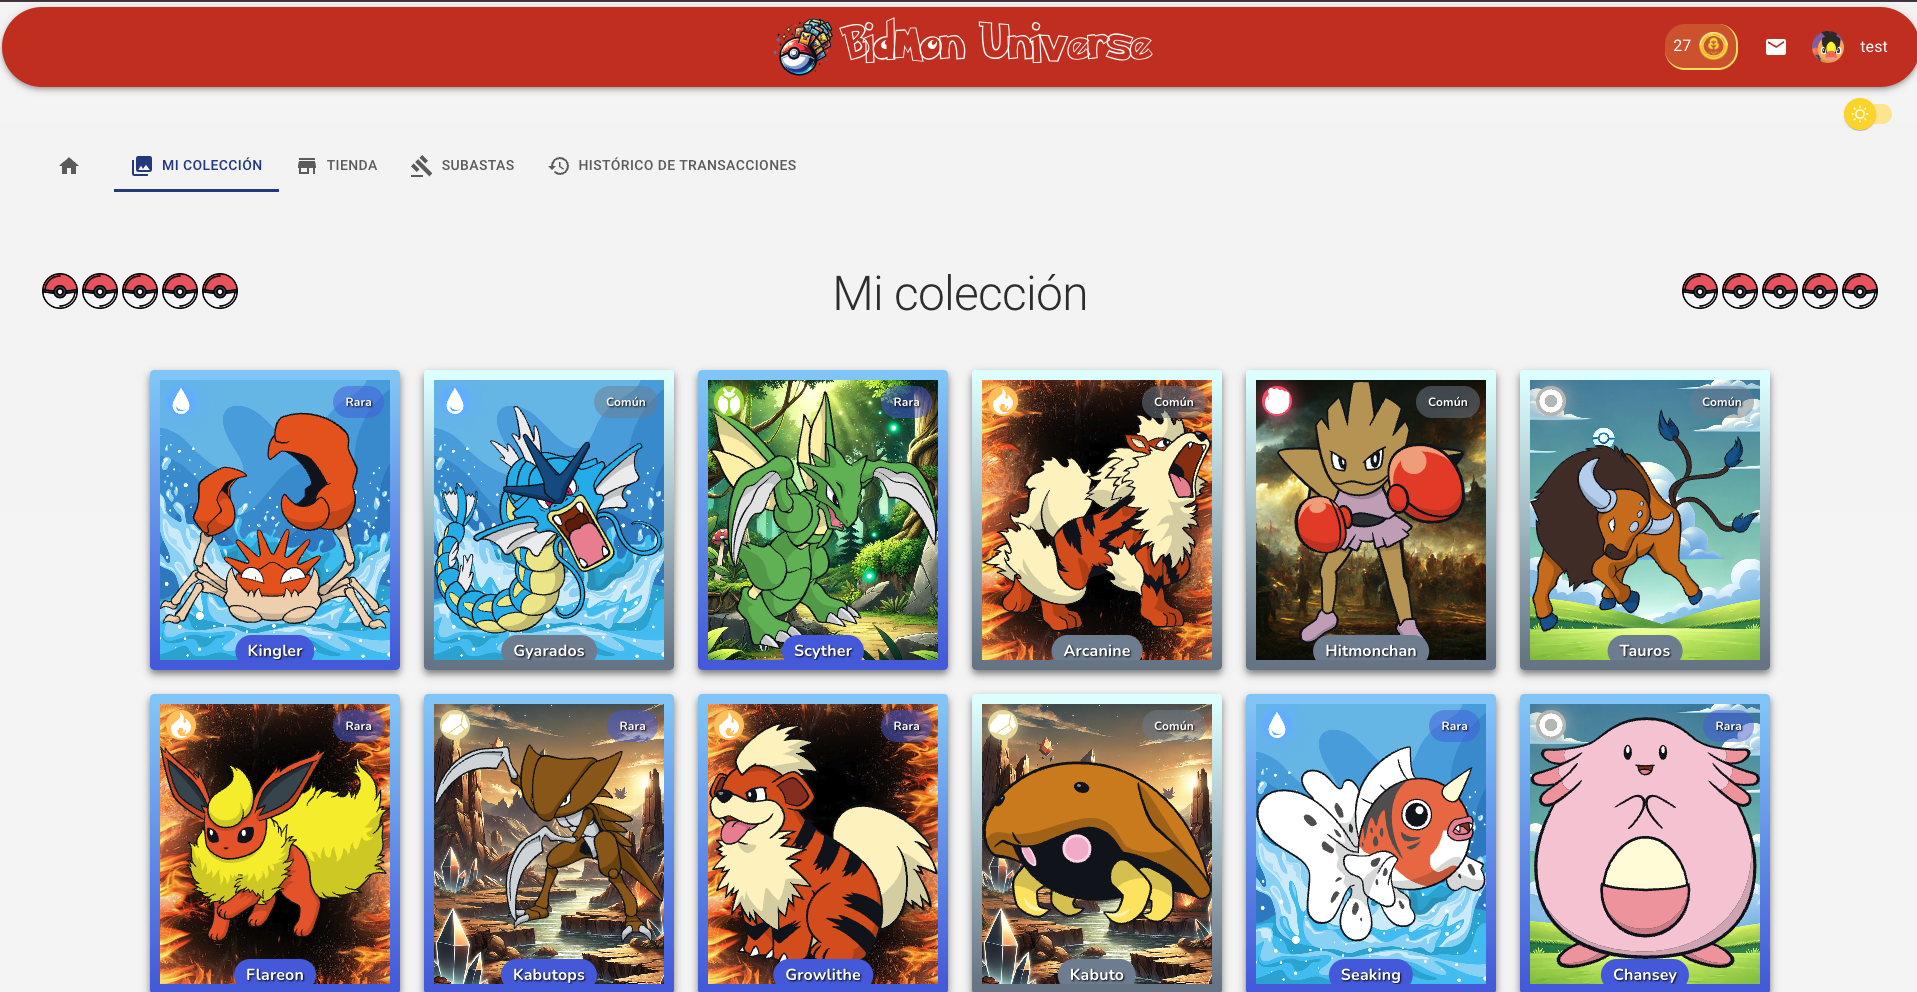
\includegraphics[width=0.8\textwidth]{figures/6-Analisis/6-Interfaz/interfaz/coleccion.png}
    \caption{Página de la colección de cartas del usuario.}
    \label{fig:m-interfaz-coleccion}
\end{figure}


\subsubsection{Crear subasta}
Para crear una subasta de una carta, el usuario debe acceder a su colección de cartas y seleccionar la carta que desea subastar.
Una vez en la página de detalle de la carta, se puede pulsar el botón de \textit{Realizar subasta} para iniciar el proceso de subasta.

\begin{figure}[H]
    \centering
    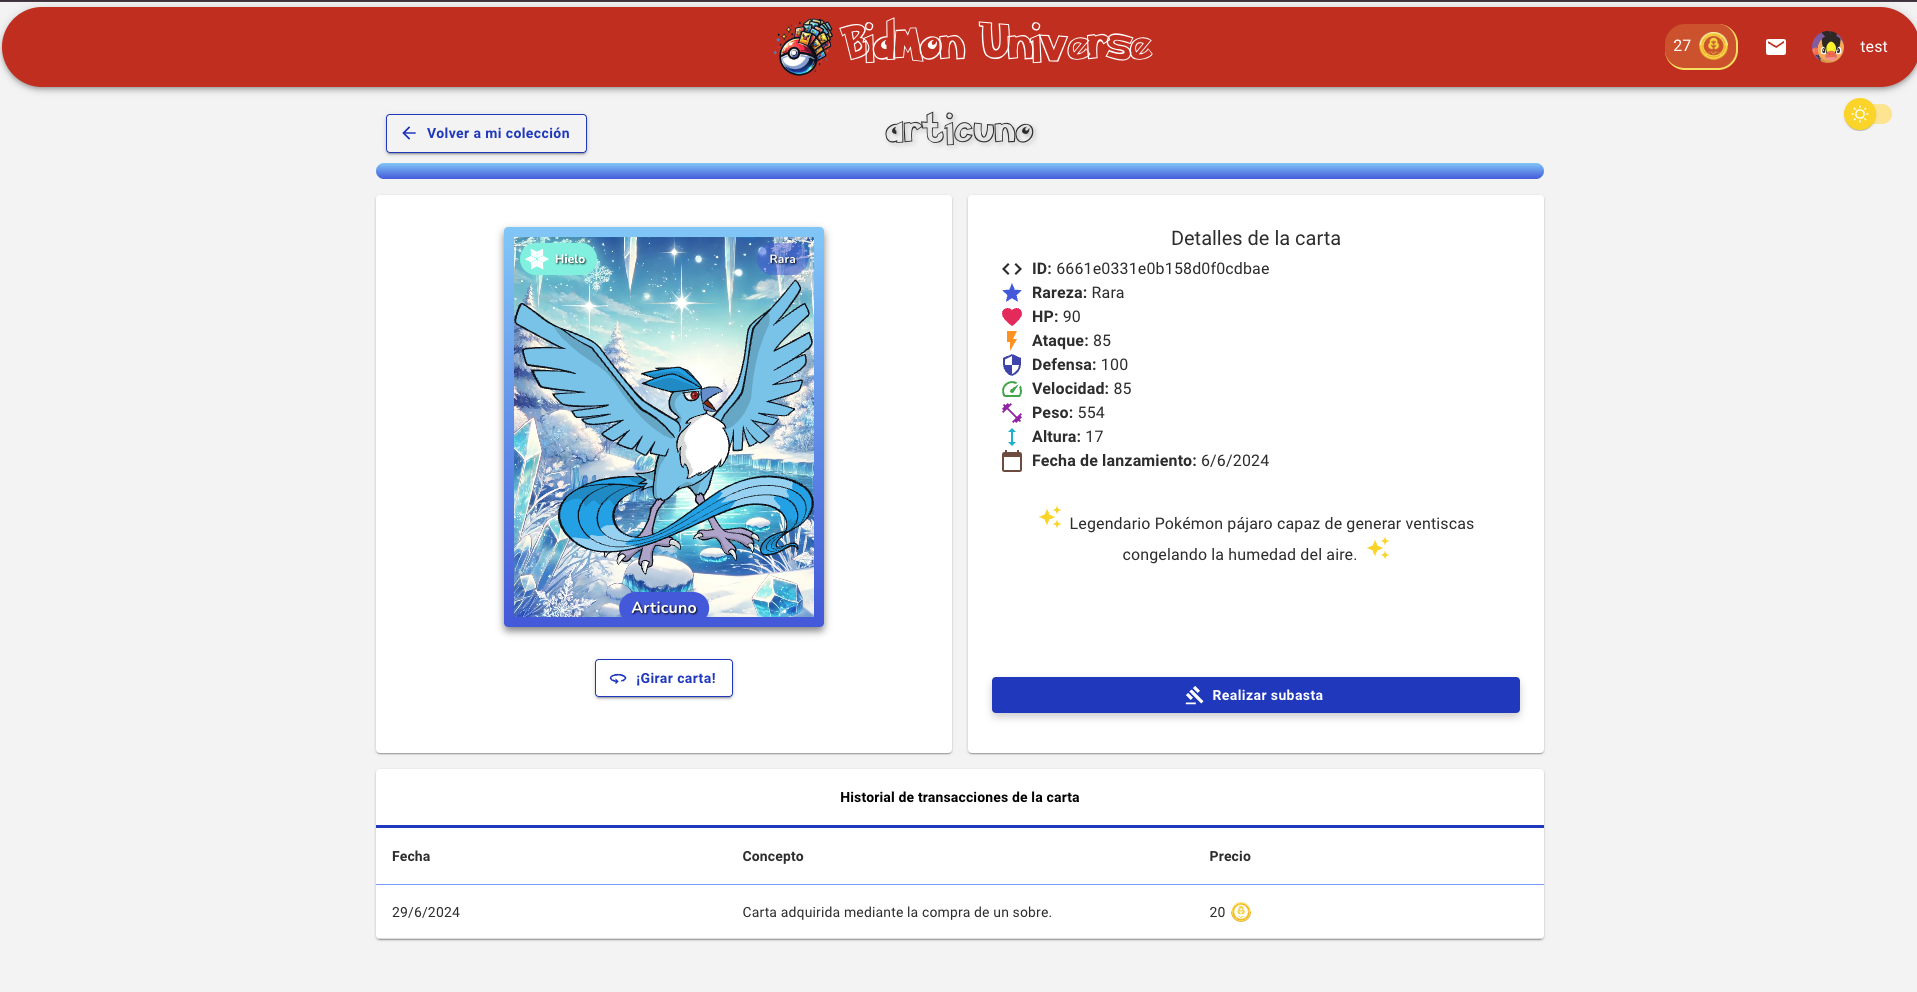
\includegraphics[width=0.8\textwidth]{figures/6-Analisis/6-Interfaz/interfaz/detalle_carta.png}
    \caption{Página de detalle de una carta de la colección del usuario.}
    \label{fig:m-interfaz-detalle-carta}
\end{figure}

El usuario debe introducir el precio de salida y la duración de la subasta. Estos son opcionales, si no se especifican, se utilizarán
valores por defecto.

\begin{figure}[H]
    \centering
    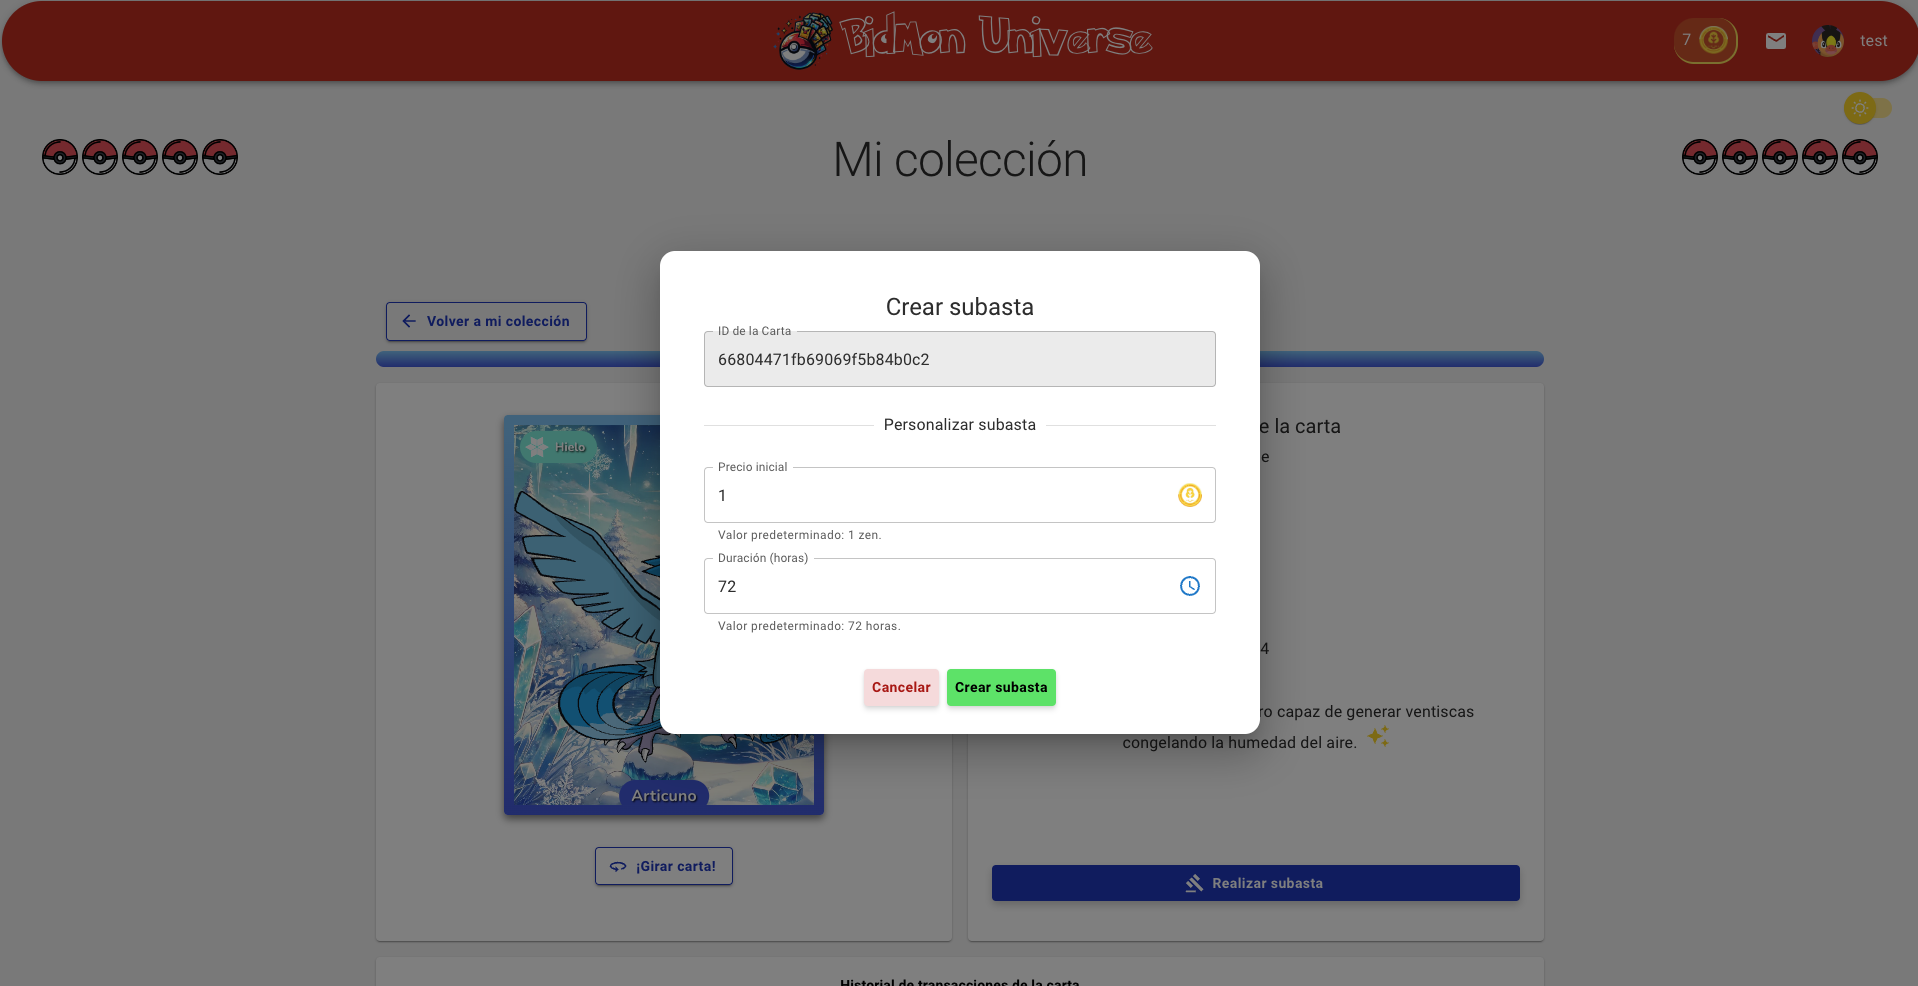
\includegraphics[width=0.8\textwidth]{figures/6-Analisis/6-Interfaz/interfaz/crear-subasta1.png}
    \caption{Modal de creación de subasta.}
    \hypertarget{fig:interfaz-subasta}{}
    \label{fig:m-interfaz-subasta}
\end{figure}


Una vez que el usuario ha rellenado los campos, puede pulsar el botón de \textit{Crear subasta} para confirmar la subasta.
Se le abrirá un modal de confirmación, en el que se le mostrará un resumen de la subasta y podrá confirmarla o cancelarla.

\subsubsection{Consultar subastas}
En la página de subastas se pueden ver todas las subastas activas de cartas.
\begin{figure}[H]
    \centering
    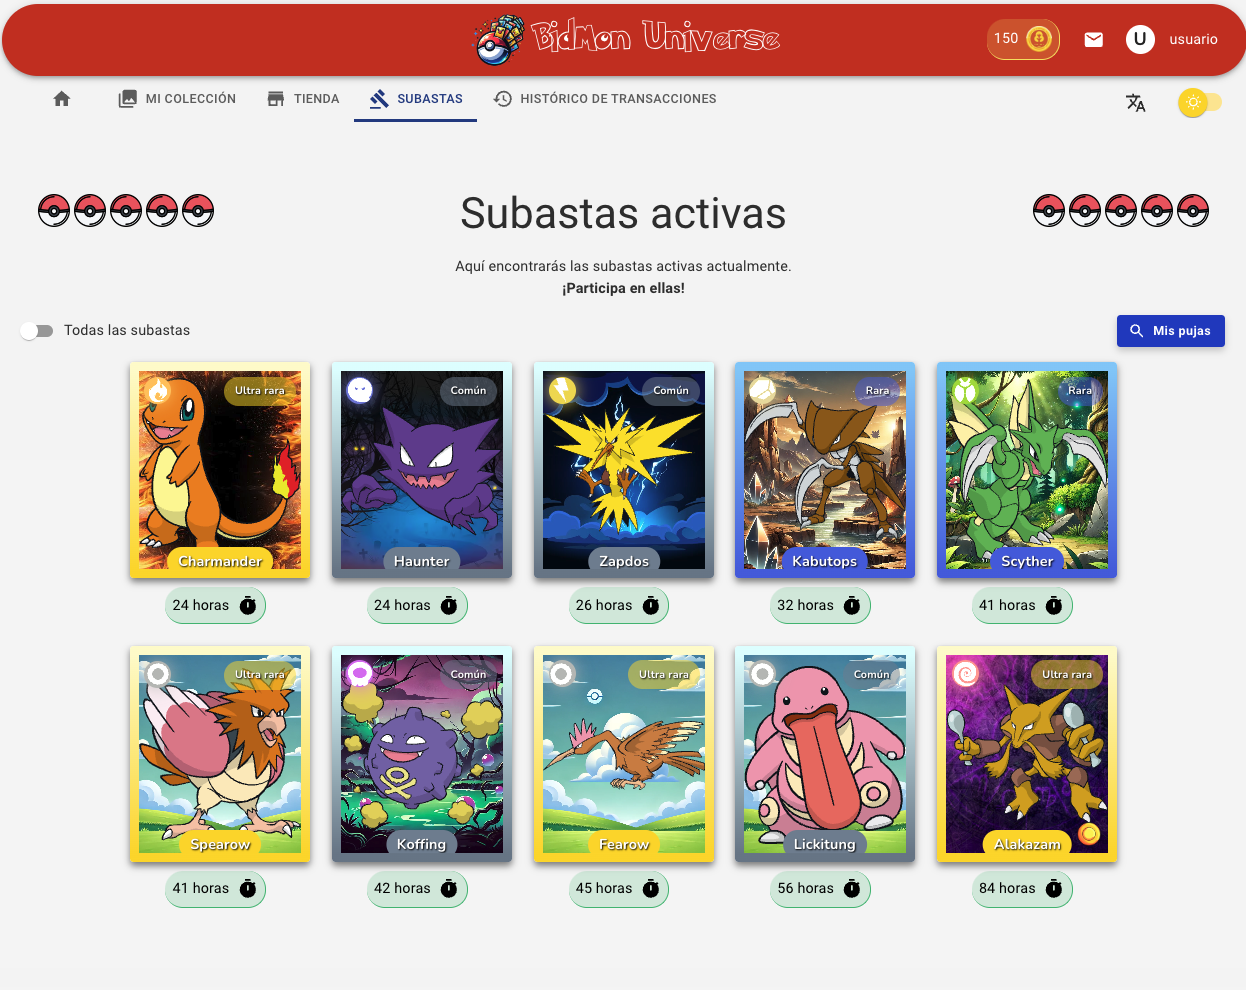
\includegraphics[width=0.8\textwidth]{figures/6-Analisis/6-Interfaz/interfaz/subastas.png}
    \caption{Página de las subastas activas de cartas.}
    \label{fig:m-interfaz-subastas}
\end{figure}

Si se hace clic en una subasta, se muestra un detalle de la subasta con información de la carta subastada y la duración restante.

\begin{figure}[H]
    \centering
    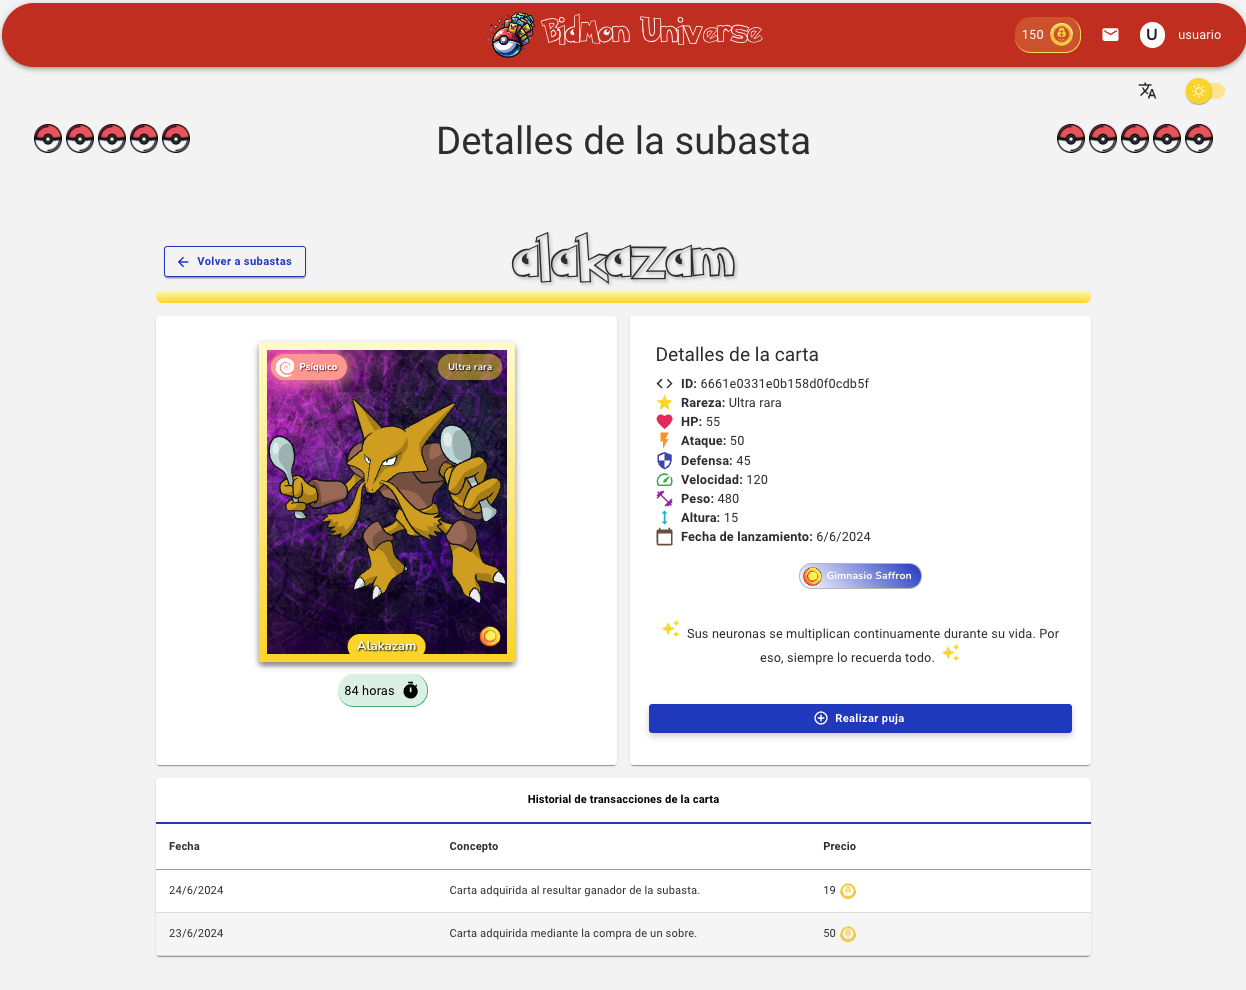
\includegraphics[width=0.8\textwidth]{figures/6-Analisis/6-Interfaz/interfaz/detalle_subasta.png}
    \caption{Página de detalle de una subasta activa.}
    \label{fig:m-interfaz-detalle-subasta}
\end{figure}


El usuario tiene la opción de pujar por la carta haciendo clic en el botón de \textit{Realizar puja} y especificando el precio de la puja.
\begin{figure}[H]
    \centering
    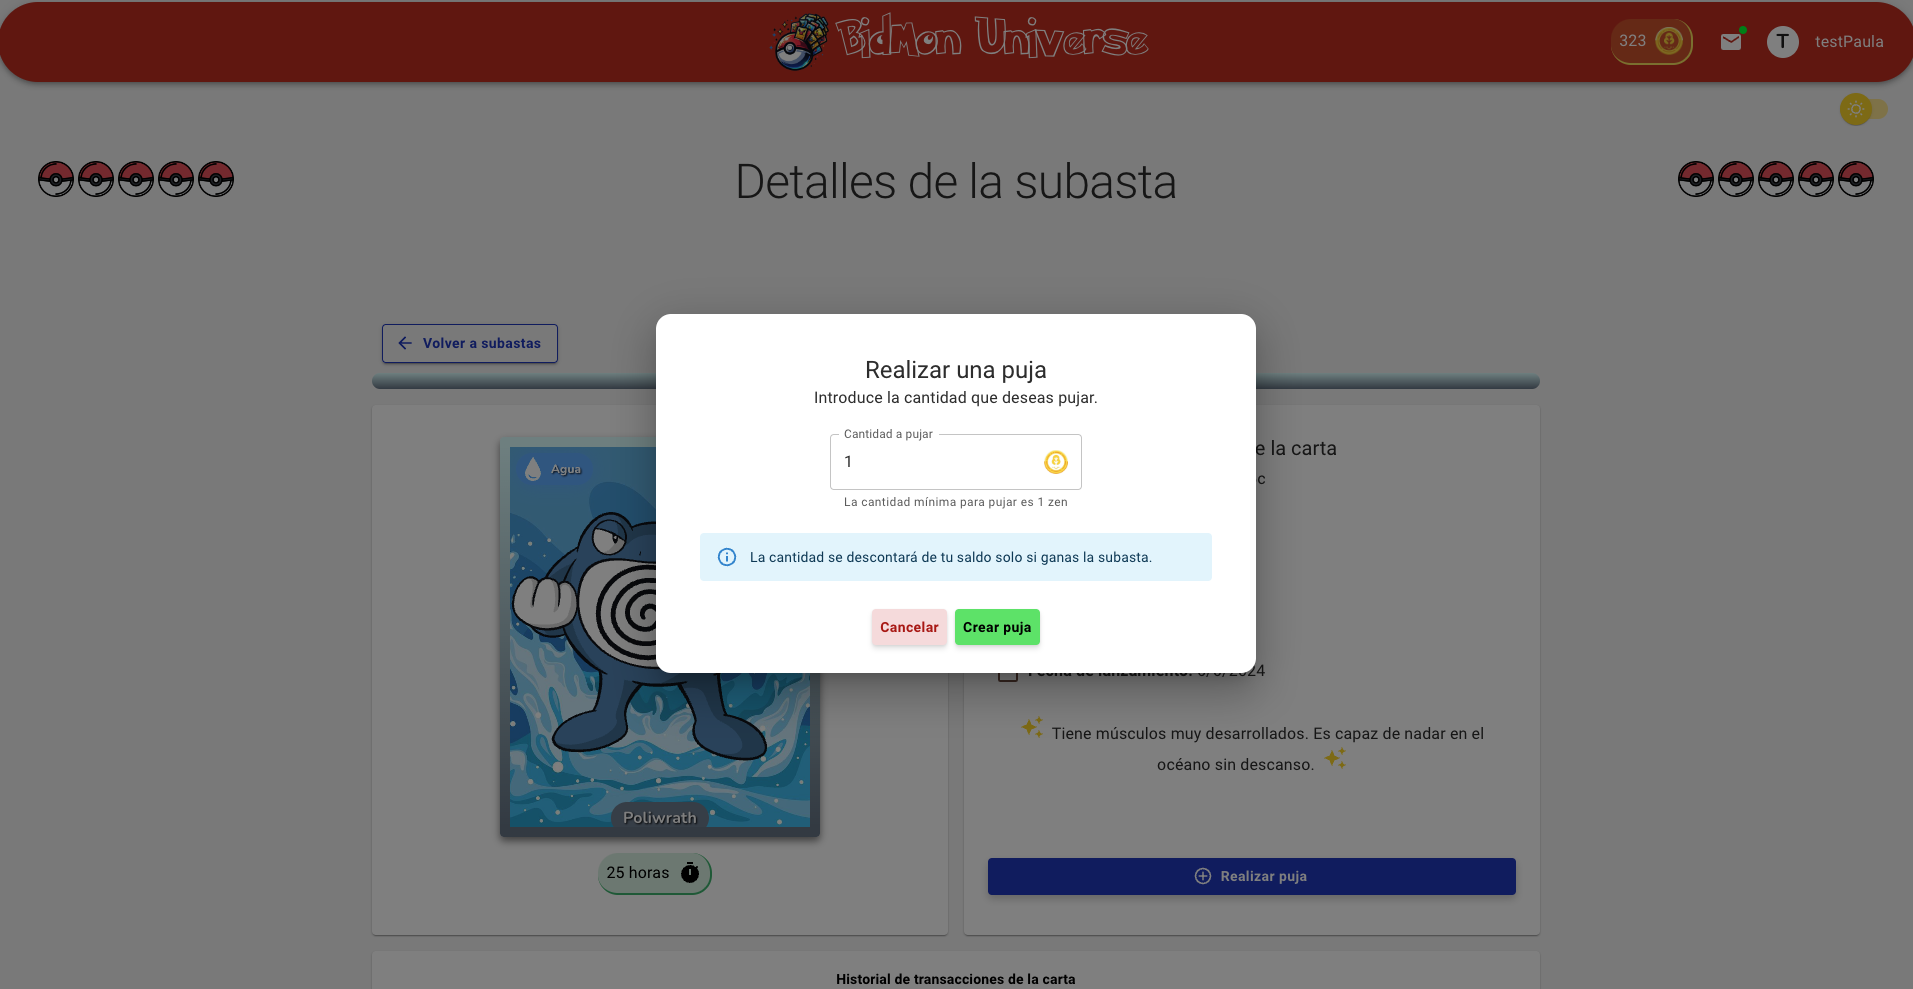
\includegraphics[width=0.8\textwidth]{figures/6-Analisis/6-Interfaz/interfaz/crear-puja.png}
    \caption{Modal de creación de puja.}
    \label{fig:m-interfaz-puja}
\end{figure}


Si el usuario ha creado una subasta, puede verla en la página de mis subastas activas.


Podría acceder al detalle de igual manera que en la página de subastas activas
y podría retirar la subasta si lo desea.

\begin{figure}[H]
    \centering
    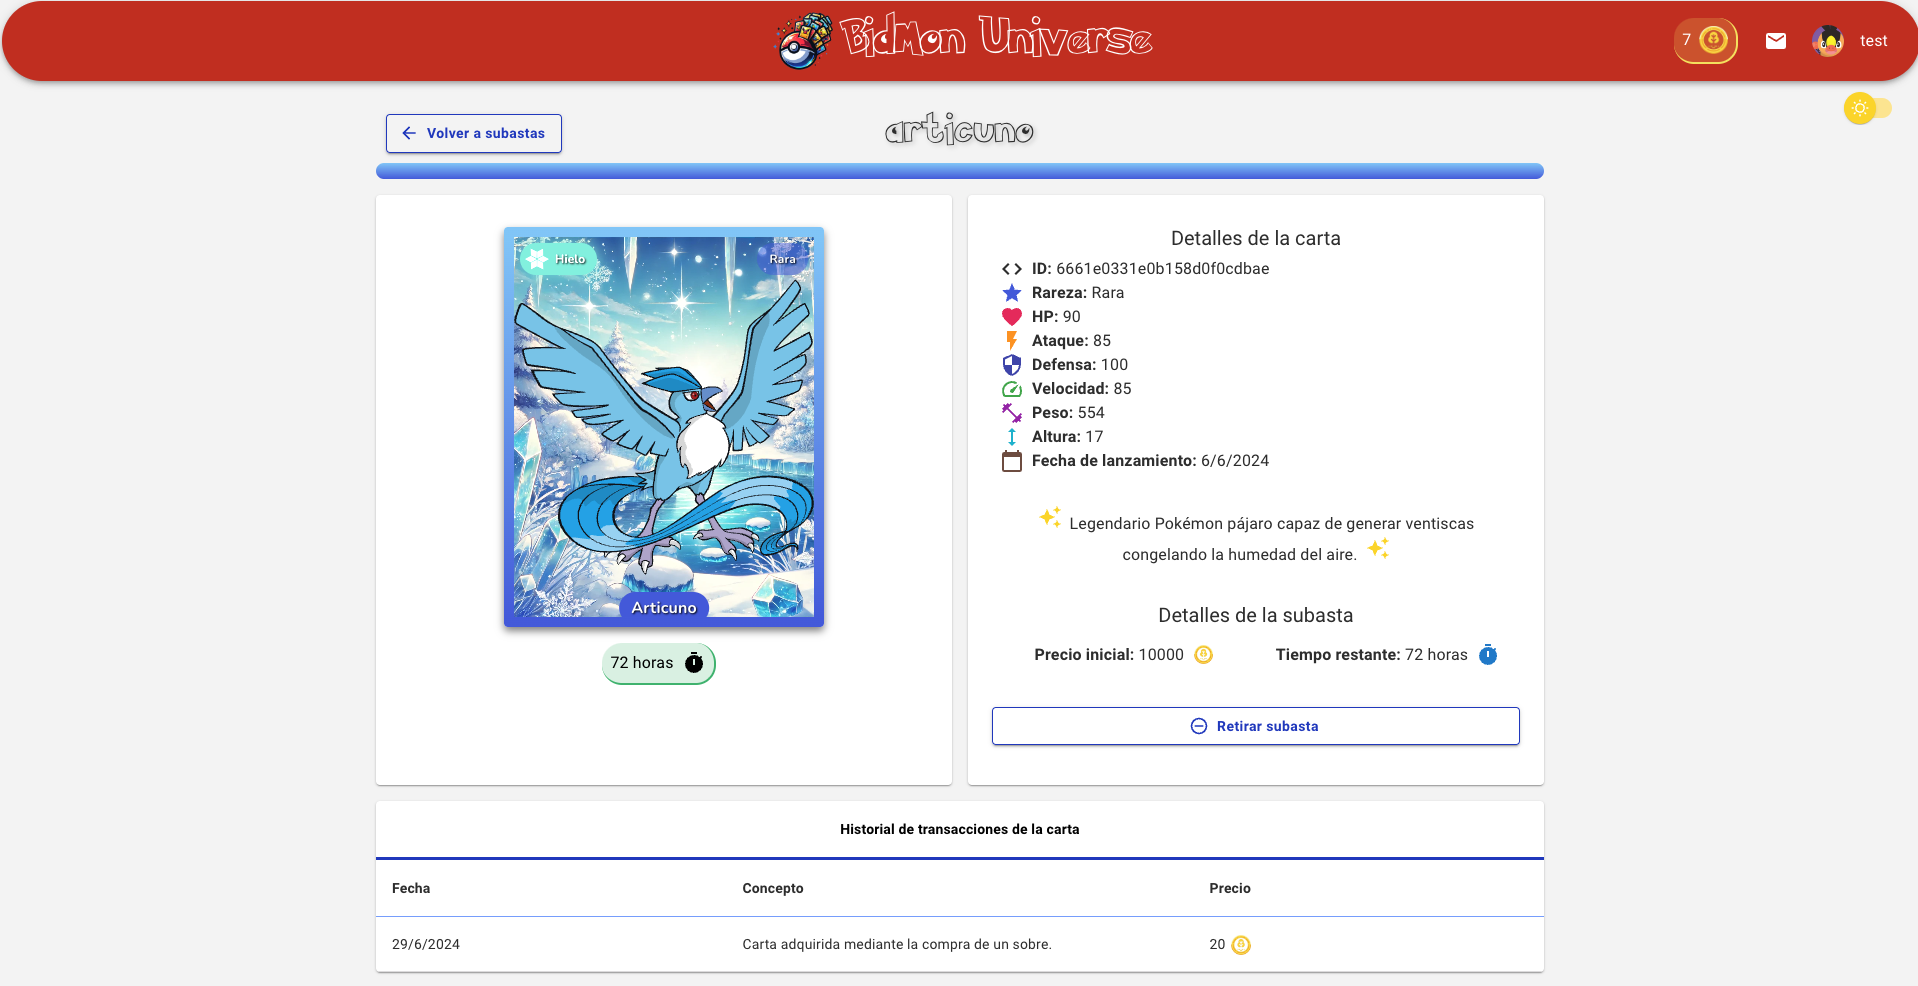
\includegraphics[width=0.8\textwidth]{figures/6-Analisis/6-Interfaz/interfaz/mi_subasta_detalle.png}
    \caption{Página de detalle de una subasta activa creada por el usuario.}
    \label{fig:interfaz-detalle-mi-subasta}
\end{figure}


\subsubsection{Consultar pujas}
En la página de subastas hay un botón \textit{Mis pujas} que lleva a una página donde se pueden ver todas las pujas activas del usuario.
\begin{figure}[H]
    \centering
    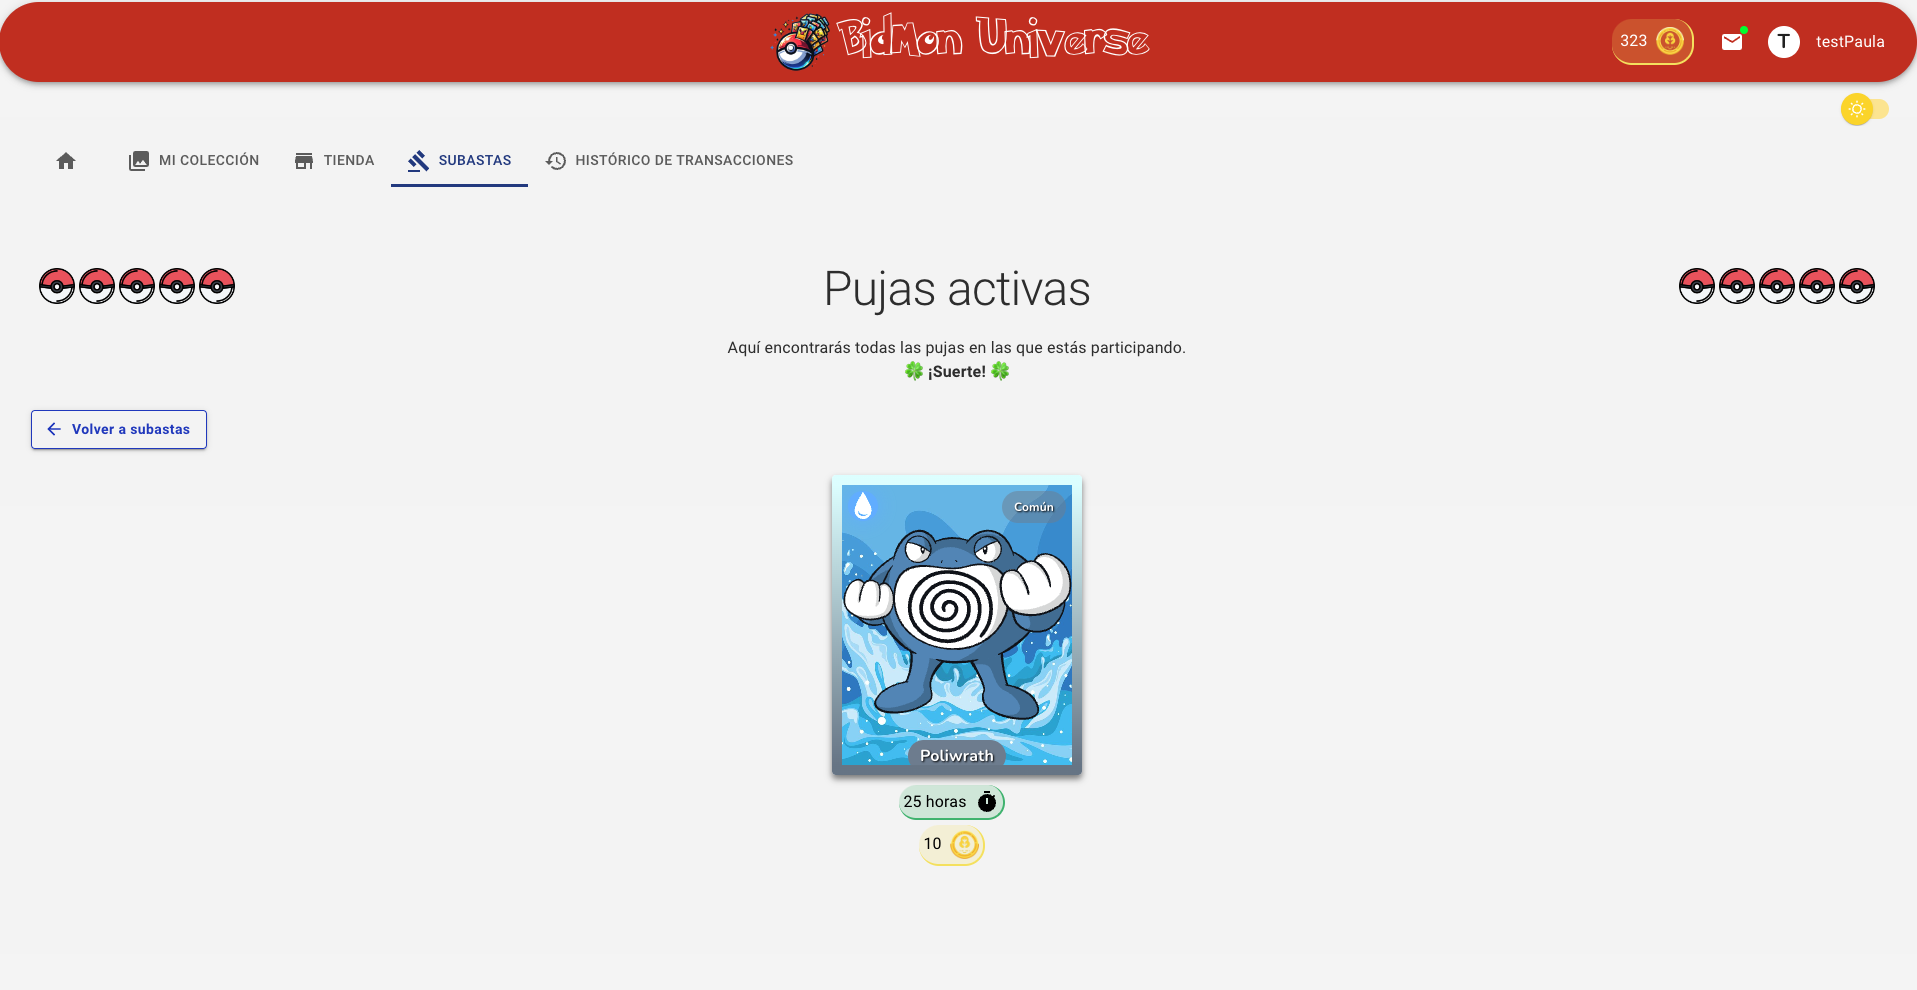
\includegraphics[width=0.8\textwidth]{figures/6-Analisis/6-Interfaz/interfaz/pujas-activas.png}
    \caption{Página de las pujas activas del usuario.}
    \label{fig:m-interfaz-mis-pujas}
\end{figure}

Si se hace clic en una puja, se muestra un detalle de la puja con información de la subasta y la carta pujada. 
El usuario tiene la opción de retirar la puja si lo desea.
\begin{figure}[H]
    \centering
    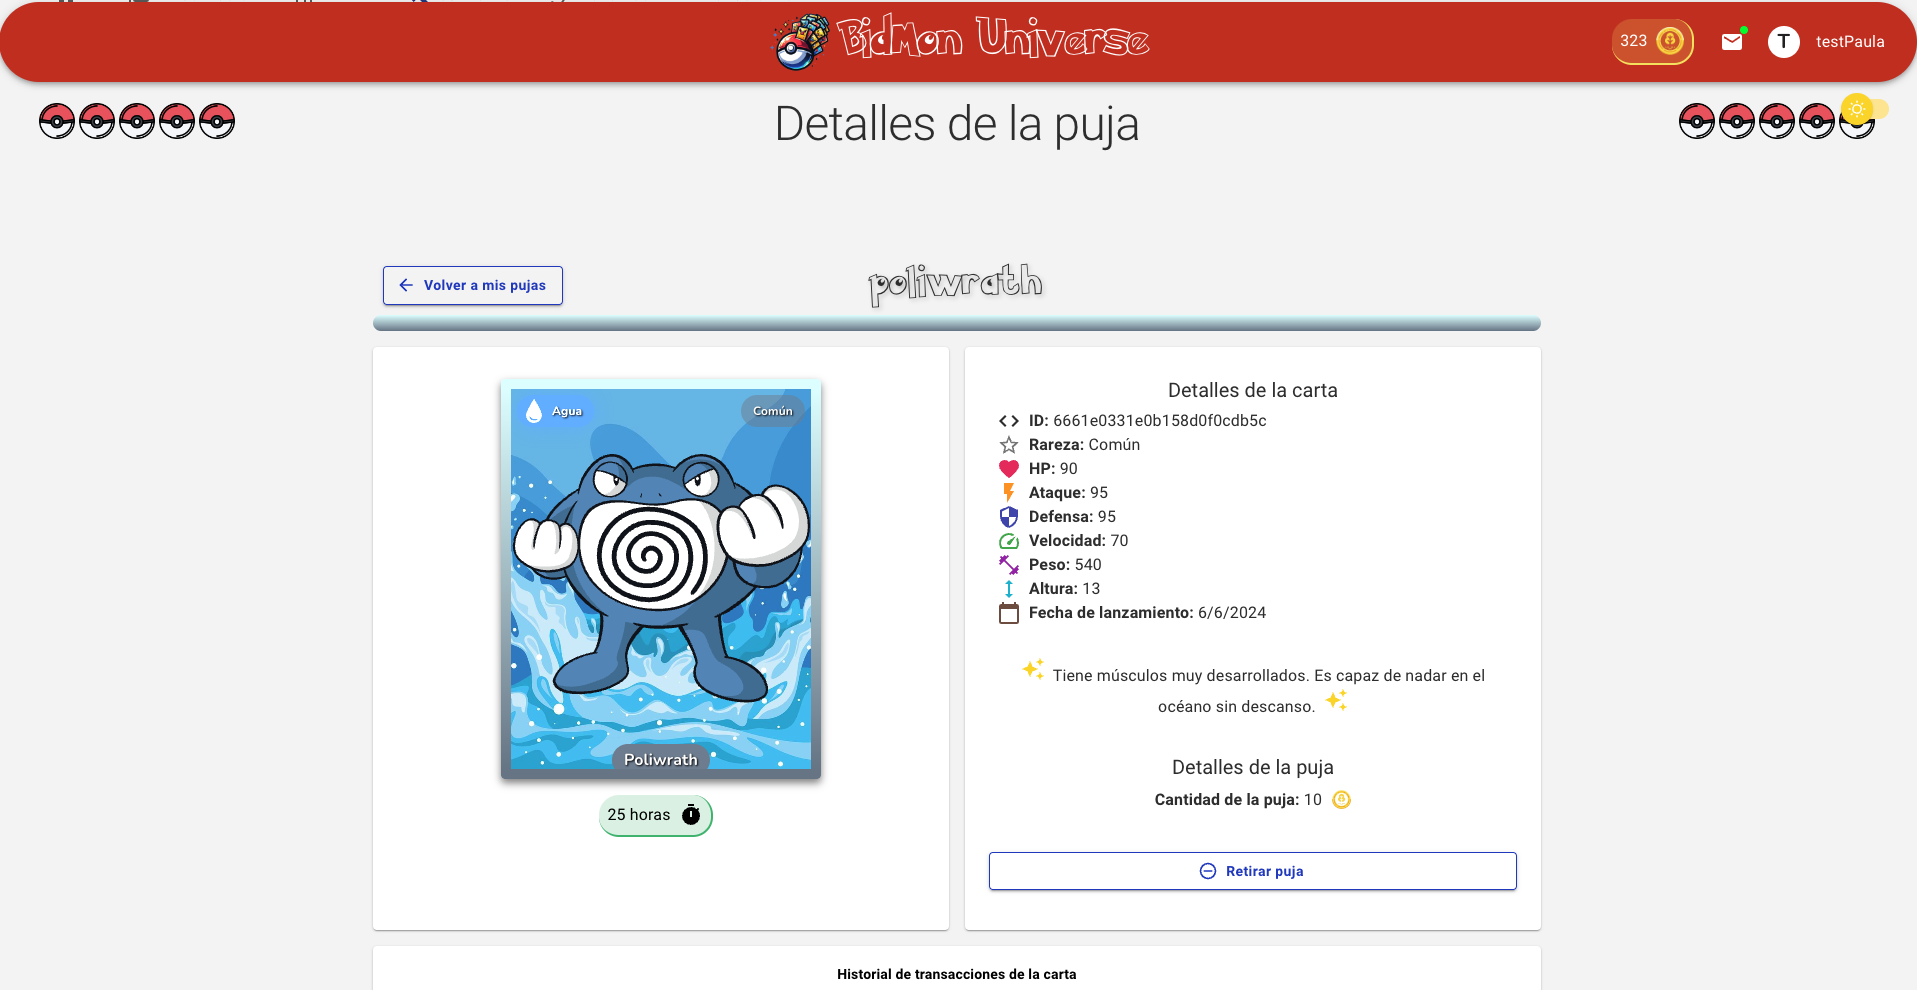
\includegraphics[width=0.8\textwidth]{figures/6-Analisis/6-Interfaz/interfaz/detalle-puja.png}
    \caption{Página de detalle de una puja activa.}
    \label{fig:m-interfaz-detalle-puja}
\end{figure}


\subsubsection{Historial de transacciones}
En la página de historial de transacciones se pueden ver todas las transacciones realizadas por el usuario.
Estas incluyen la compra de sobres y todos los movimientos de cartas realizados en subastas, es decir,
las pujas y subastas realizadas por el usuario.

\begin{figure}[H]
    \centering
    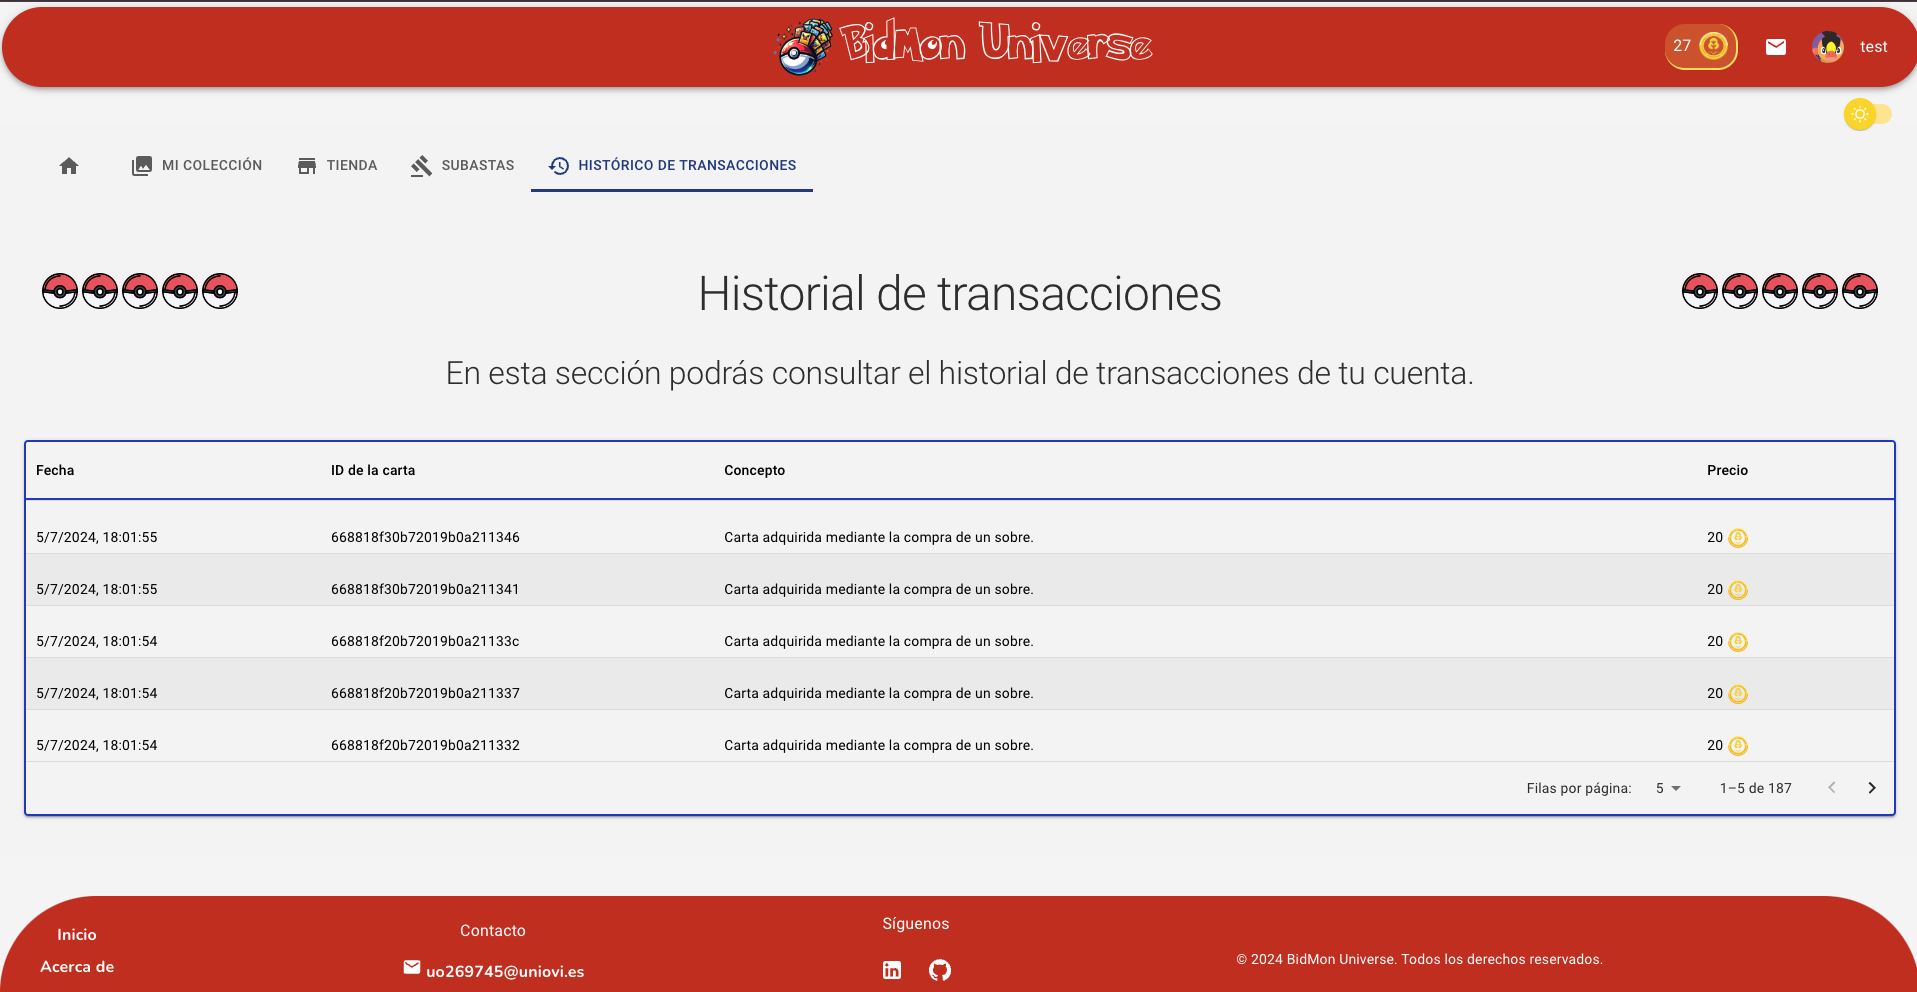
\includegraphics[width=0.8\textwidth]{figures/6-Analisis/6-Interfaz/interfaz/transacciones.png}
    \caption{Página de transacciones realizadas por el usuario.}
    \label{fig:interfaz-transacciones}
\end{figure}


\subsubsection{Recarga de saldo}
En la página de recarga de saldo se puede recargar el saldo de la aplicación con dinero real.
A esta página se accede desde el botón que muestra el saldo en la esquina superior derecha de la aplicación.
Para ello se utiliza la pasarela de pago de PayPal, que permite realizar pagos de forma segura y sencilla.
La equivalencia entre Zens y dinero real es de 1 Zens = 0,01 €.
El mínimo de recarga es de 10 Zens y todas las recargas deben de ser múltiplos de 10.

\begin{figure}[H]
    \centering
    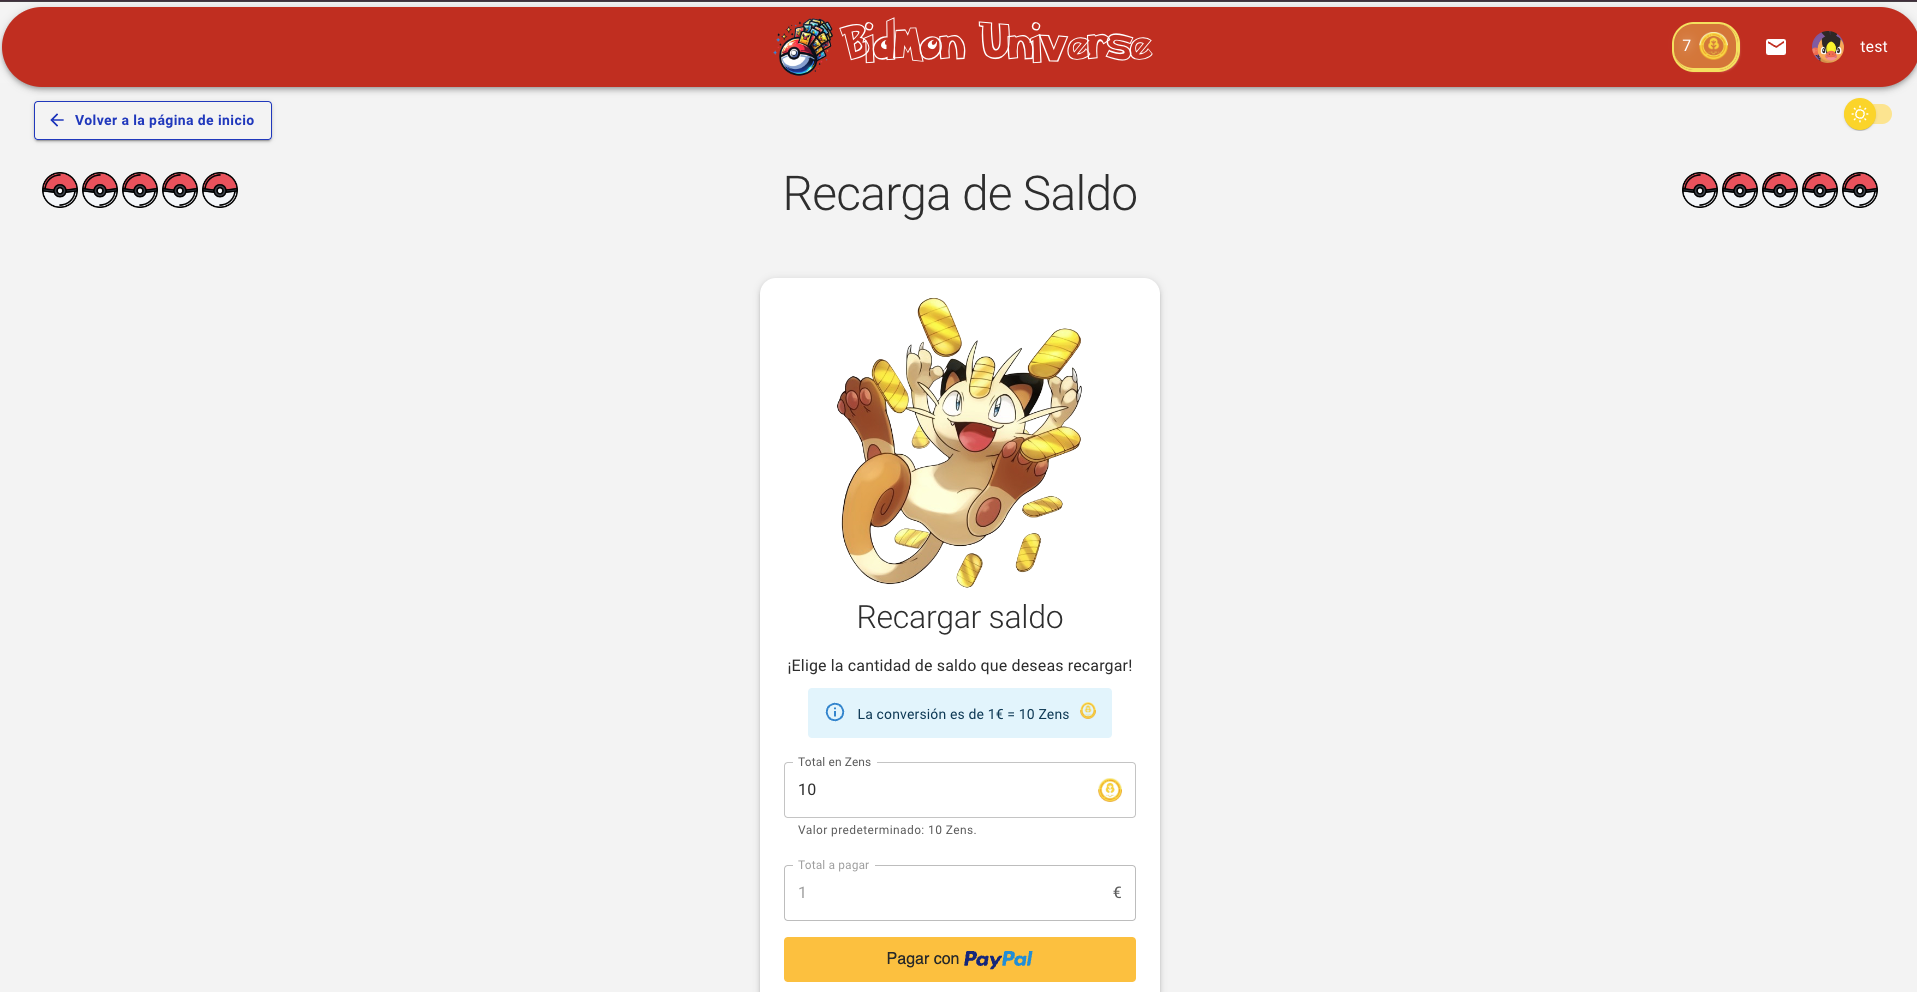
\includegraphics[width=0.8\textwidth]{figures/6-Analisis/6-Interfaz/interfaz/recarga.png}
    \caption{Página de recarga de saldo de la aplicación.}
    \label{fig:m-interfaz-recarga}
\end{figure}

\subsubsection{Consultar notificaciones}
En la esquina superior derecha de la aplicación hay un icono de sobre a través del cual se pueden consultar las notificaciones.
Si el usuario tiene notificaciones pendientes, se mostrará un indicador en el icono.
\begin{figure}[H]
    \centering
    
\includegraphics[width=0.4\textwidth]{figures/6-Analisis/6-Interfaz/interfaz/notificaciones_1.png}
    \caption{Indicador de notificaciones pendientes.}
    \label{fig:m-interfaz-notificaciones1}
\end{figure}
Las notificaciones pueden ser de diferentes tipos, si están catalogadas como importantes, se mostrará un icono de una campana en color rojo.
Si son notificaciones normales, no se mostrará ningún icono.

\begin{figure}[H]
    \centering
    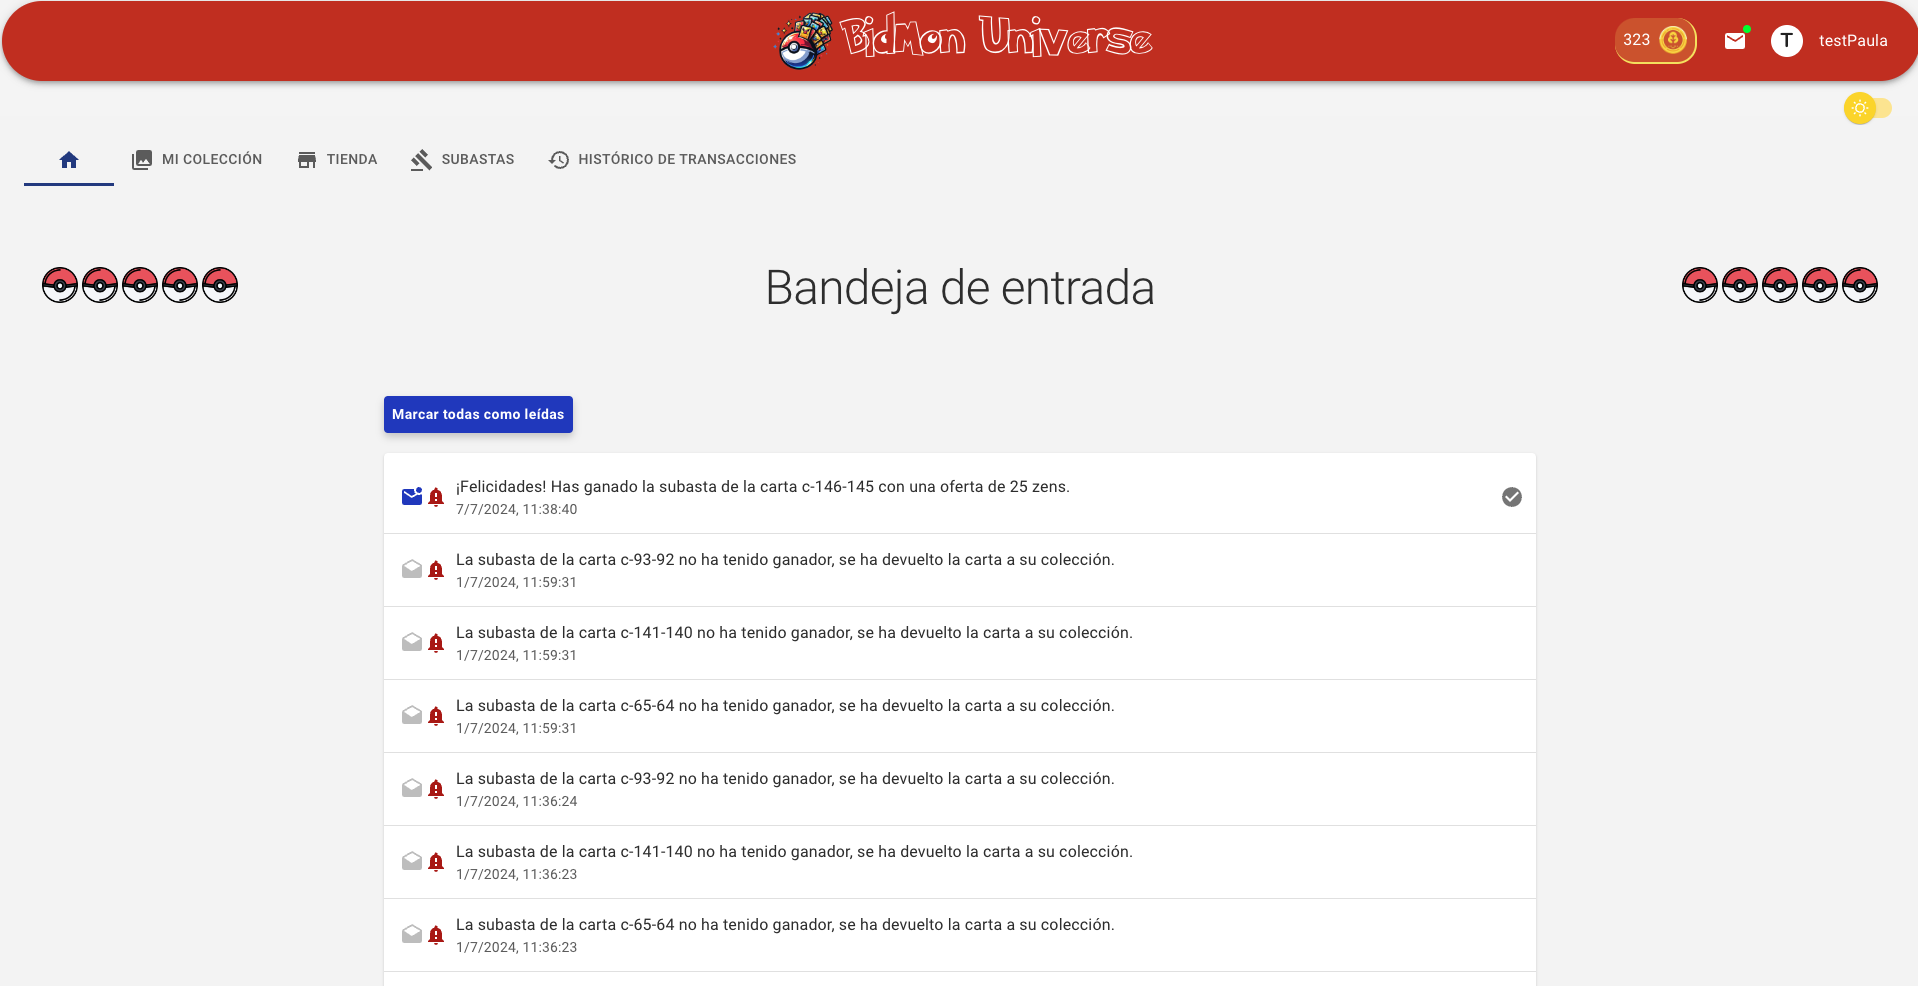
\includegraphics[width=0.8\textwidth]{figures/6-Analisis/6-Interfaz/interfaz/notificaciones_2.png}
    \caption{Página de notificaciones del usuario.}
    \label{fig:m-interfaz-notificaciones2}
\end{figure}


\subsubsection{Perfil de usuario}
En la página de perfil de usuario se pueden ver los datos del usuario, como el nombre de usuario y la imagen de perfil.
El usuario puede cambiar su imagen de perfil y su contraseña desde esta página.
A esta página se accede haciendo clic en el avatar del usuario en la esquina superior derecha de la aplicación.

\begin{figure}[H]
    \centering
    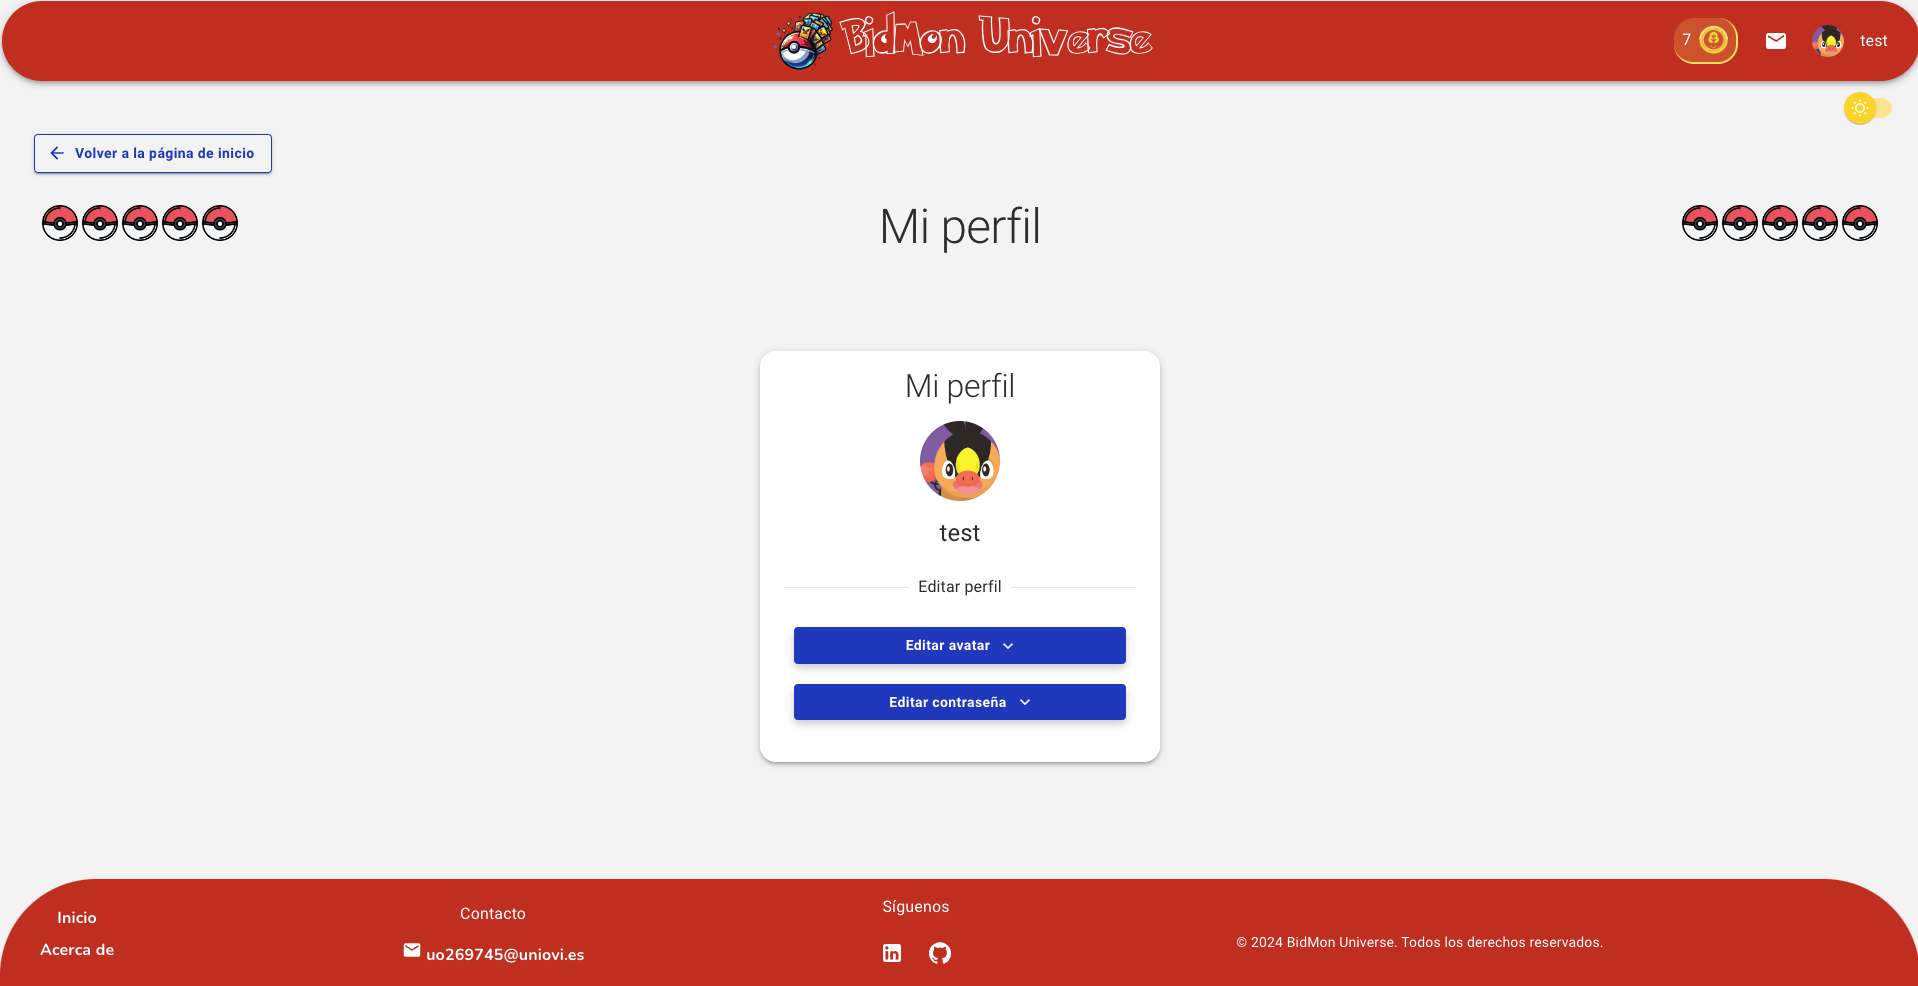
\includegraphics[width=0.8\textwidth]{figures/6-Analisis/6-Interfaz/interfaz/perfil1.png}
    \caption{Página de perfil del usuario.}
    \label{fig:interfaz-perfil1}
\end{figure}


\begin{figure}[H]
    \centering
    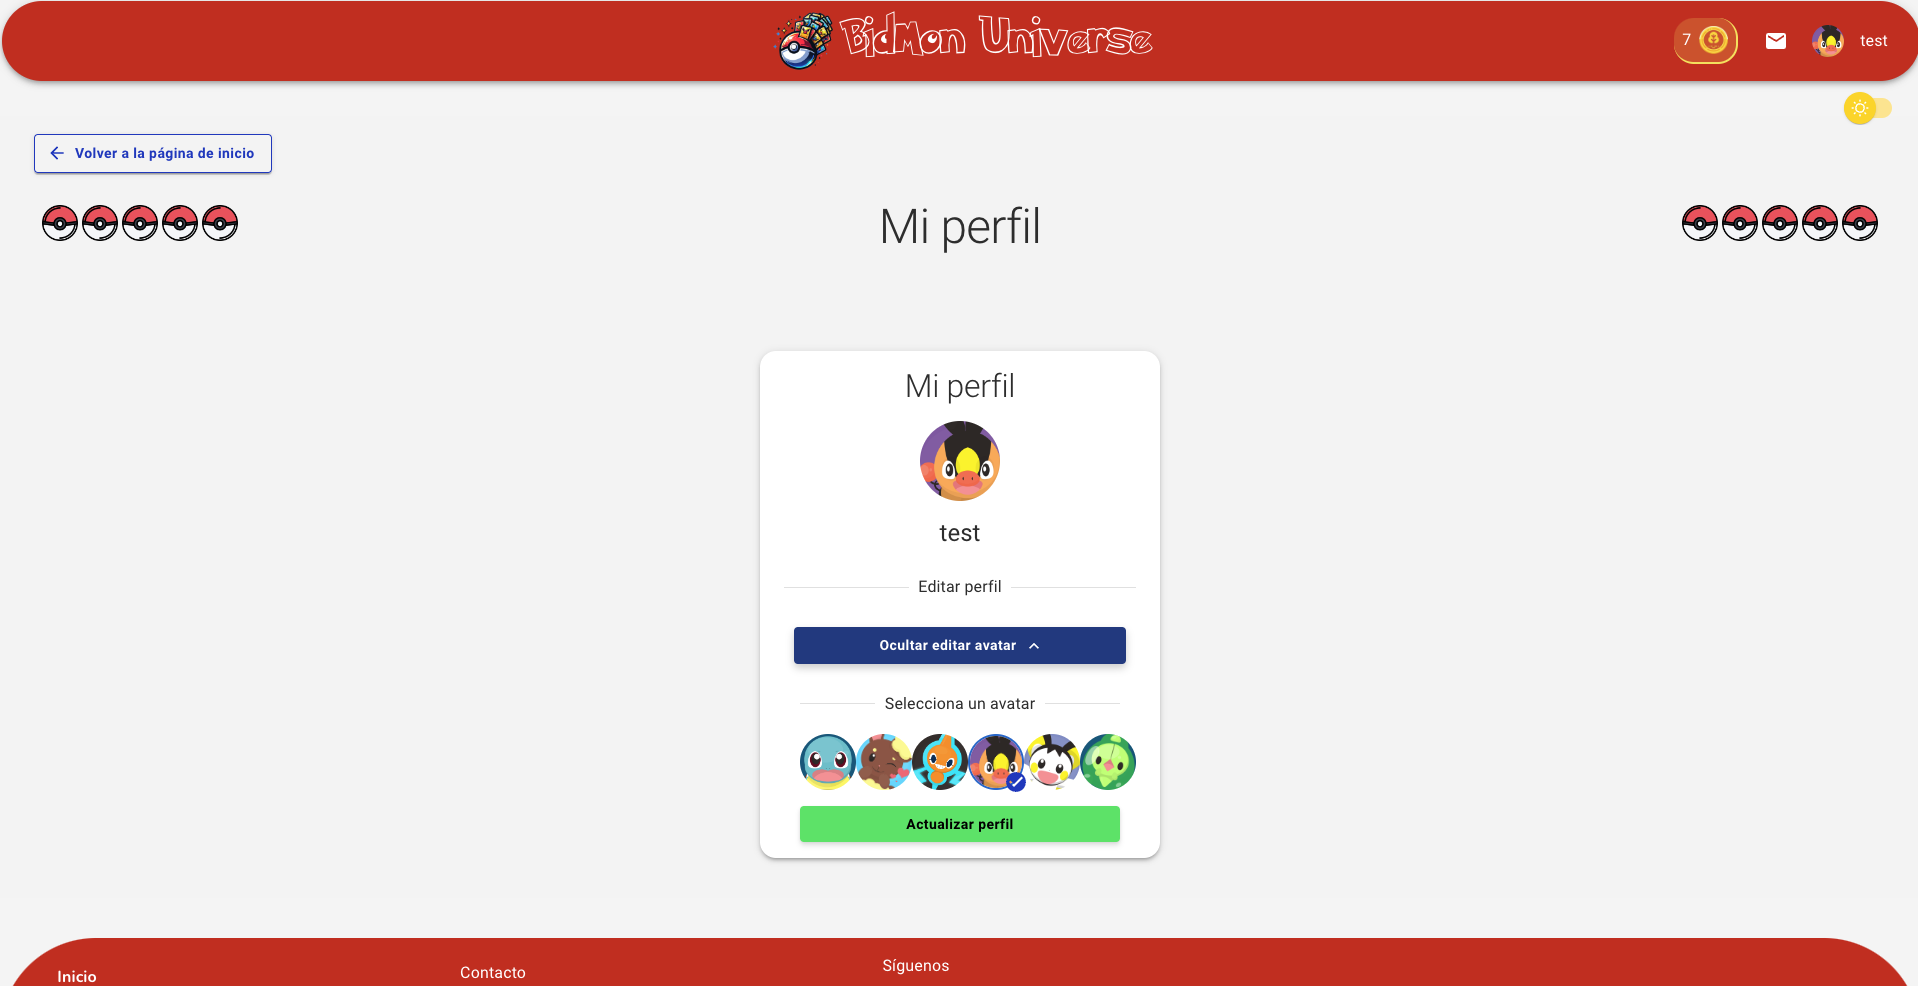
\includegraphics[width=0.8\textwidth]{figures/6-Analisis/6-Interfaz/interfaz/perfil2.png}
    \caption{Página de perfil del usuario, con la opción de cambiar la imagen de perfil desplegada.}
    \label{fig:interfaz-perfil2}
\end{figure}

Es importante que el usuario recuerde su contraseña, ya que no se puede recuperar en caso de olvido.
Además, debe asegurarse de confirmar los cambios antes de salir de la página de perfil, ya que los cambios no se guardarán si no se confirman.

\subsubsection{Cierre de sesión}
Para cerrar la sesión, el usuario puede hacer clic sobre  su avatar en la esquina superior derecha y seleccionar la opción de \textit{Cerrar sesión}.







\newpage
\section{CARGA INICIAL DE DATOS}
Si se requiere una carga inicial de datos en la base de datos, se puede realizar mediante un script de importación de datos.
Este script puede leer los datos de un archivo CSV y cargarlos en la base de datos del sistema.
También se puede utilizar un script de exportación de datos para generar un archivo CSV con datos para inicializar la base de datos.

Estos scripts se ejecutarán localmente dependiendo de los datos que se quieran importar o exportar.
Los archivos generados deben de estar en el directorio \texttt{data} de la carpeta \texttt{restapi}.
Es necesario tener instalado Node.js y npm en el sistema para ejecutar los scripts y comprobar que la base de datos está en funcionamiento.
Además, si se realiza una importanción con datos recopilados manualmente, es necesario que los datos estén en el formato correcto.
Para ejecutar los scripts, se debe situar en la carpeta \texttt{restapi} y ejecutar los siguientes comandos:
\begin{itemize}
    \item Exportar datos de cartas:
    \begin{enumerate}
        \item \texttt{npm run fetch-data}
        \item Este comando generará un archivo \texttt{cards\_data.csv} en el directorio \texttt{data}. Recopila datos de PokéAPI
        \coloredUnderline{\href{https://pokeapi.co/}{PokéAPI}}, aplica la lógica de negocio y los exporta a un archivo CSV.
    \end{enumerate}
    \item Importar datos de cartas:
    \begin{enumerate}
        \item \texttt{npm run load-data}
        \item Este comando leerá el archivo \texttt{cards\_data.csv} y cargará los datos en la base de datos.
    \end{enumerate}
    \item Exportar datos de mazos:
    \begin{enumerate}
        \item \texttt{npm run fetchDecksData}
        \item Este comando generará un archivo \texttt{decks\_data.csv} en el directorio \texttt{data}.
    \end{enumerate}
    \item Importar datos de mazos:
    \begin{enumerate}
        \item \texttt{npm run loadDecksData}
        \item Este comando leerá el archivo \texttt{decks\_data.csv} y cargará los datos en la base de datos.
    \end{enumerate}
    \item Importar datos de sobres de cartas:
    \begin{enumerate}
        \item \texttt{npm run loadCardPacksData}
        \item Este comando leerá el archivo \texttt{cardPacks\_data.csv} y cargará los datos en la base de datos.
    \end{enumerate}
\end{itemize}
